\documentclass[UTF8,11pt,a4paper]{ctexart}

% --------------------------------------------------
% 宏包
% --------------------------------------------------
\usepackage[margin=2.2cm]{geometry}
\usepackage{amsmath,amssymb,mathtools}
\usepackage{graphicx}
\usepackage{subcaption}
\usepackage{booktabs}
\usepackage{array}
\usepackage{multirow}
\usepackage{siunitx}
\usepackage{microtype}
\usepackage{enumitem}
\usepackage{xcolor}
\usepackage{hyperref}
\usepackage{fancyhdr}
\usepackage{float}
\usepackage{placeins}

\graphicspath{{figures/}}
\sisetup{scientific-notation=true,round-mode=figures,round-precision=4}

\hypersetup{
    colorlinks=true,
    linkcolor=blue!45!black,
    citecolor=blue!45!black,
    urlcolor=blue!45!black,
    pdftitle={预设电磁场中单粒子漂移的数值模拟},
    pdfauthor={Juan Pablo Solís Ruiz}
}

\pagestyle{fancy}
\fancyhf{}
\lhead{单粒子漂移模拟}
\rhead{等离子体物理基础}
\cfoot{\thepage}
\setlength{\headheight}{14pt}

\newcommand{\vect}[1]{\boldsymbol{#1}}
\newcommand{\vE}{\vect{v}_{E}}
\newcommand{\vgradB}{\vect{v}_{\nabla B}}
\newcommand{\vc}{\vect{v}_{c}}
\newcommand{\vp}{\vect{v}_{p}}
\newcommand{\Ohm}{\Omega_c}
\newcommand{\rhL}{\rho_L}

\begin{document}

% --------------------------------------------------
% 封面
% --------------------------------------------------
\begin{titlepage}
    \centering
    \vspace*{2.0cm}

    {\Large 中国科学技术大学（USTC）\par}
    \vspace{1.1cm}

    {\huge\bfseries 预设电磁场中单粒子漂移的\par}
    \vspace{0.25cm}
    {\huge\bfseries 数值模拟\par}

    \vspace{1.4cm}
    {\Large 等离子体物理基础\par}

    \vfill

    \begin{tabular}{rl}
        \textbf{学生：} & Juan Pablo Solís Ruiz \\
        \textbf{专业：} & 物理学硕士——等离子体物理 \\
        \textbf{方法：} & C++17 全轨道积分 + Python 验证 \\
	\textbf{代码仓库：} & \url{https://github.com/h4xter1612/charged_particle_sim} \\
        \textbf{日期：} & 2026年10月
    \end{tabular}

    \vfill
\end{titlepage}

\section*{摘要}
本文实现了一个三维带电粒子全轨道模拟程序，用于研究预设电磁场中的单粒子漂移运动。程序采用 C++17 编写，并使用经典四阶 Runge--Kutta 方法对归一化后的洛伦兹方程进行数值积分；随后利用独立的 Python 脚本进行解析解比较、导引中心诊断、守恒量检验以及可视化。本文直接从完整的洛伦兹动力学中再现了五种要求的漂移：$E\times B$ 漂移、磁场梯度漂移、曲率漂移、空间非均匀电场漂移以及极化漂移。在引入非均匀场之前，首先使用匀强磁场算例验证数值积分器。对于存在精确解析解的算例，数值全轨道解与解析解的误差约为 $10^{-9}$--$10^{-11}$；对于非均匀场算例，数值结果则再现了预期的导引中心理论以及有限拉莫尔半径修正。

\tableofcontents
\newpage

% --------------------------------------------------
\section{研究目标与范围}
% --------------------------------------------------

本项目的目标是在给定电磁场中直接模拟带电粒子的完整轨道，并从洛伦兹动力学中恢复课堂所讨论的漂移运动。要求研究的五种情形为
\begin{enumerate}[label=\arabic*.]
    \item 匀强正交电磁场中的 $\vect{E}\times\vect{B}$ 漂移；
    \item 磁场梯度（$\nabla B$）漂移；
    \item 曲率漂移；
    \item 空间非均匀电场中的漂移；
    \item 随时间变化电场中的极化漂移。
\end{enumerate}

另外增加一个匀强磁场算例，用于在引入任何产生漂移的非均匀性之前验证数值方法。C++ 程序直接积分完整的洛伦兹力方程，并未把任何漂移速度人为加入运动方程。之后，Python 脚本读取生成的 CSV 轨迹，并与解析解或导引中心理论比较，同时检验守恒关系并生成本文中的图像。

% --------------------------------------------------
\section{物理模型与归一化}
% --------------------------------------------------

\subsection{洛伦兹方程}

对于质量为 $m$、电荷为 $q$ 的粒子，其有量纲运动方程为
\begin{align}
    \frac{d\vect{r}}{dt} &= \vect{v}, \\
    m\frac{d\vect{v}}{dt} &= q\left[\vect{E}(\vect{r},t)+\vect{v}\times\vect{B}(\vect{r},t)\right].
    \label{eq:lorentz_dimensional}
\end{align}
磁洛伦兹力始终垂直于粒子的瞬时速度，因此磁场本身不对粒子做功。当 $\vect{E}=0$ 时，动能应保持不变；当存在静电场或随时间变化的电场时，则采用相应的总能量或功--能关系进行检验。

\subsection{无量纲变量}

所有模拟均在归一化单位下进行。取 $B_{\rm ref}$、$v_{\rm ref}$、$m_{\rm ref}$ 和 $|q_{\rm ref}|$ 为参考量，并定义
\begin{equation}
    \Omega_{\rm ref}=\frac{|q_{\rm ref}|B_{\rm ref}}{m_{\rm ref}},
    \qquad
    t_{\rm ref}=\Omega_{\rm ref}^{-1},
    \qquad
    \rho_{\rm ref}=\frac{v_{\rm ref}}{\Omega_{\rm ref}},
    \qquad
    E_{\rm ref}=v_{\rm ref}B_{\rm ref}.
\end{equation}
其中 $\Omega_{\rm ref}$ 是由参考粒子和参考磁场定义的参考回旋频率，$t_{\rm ref}$ 是相应的时间尺度，$\rho_{\rm ref}$ 是参考拉莫尔半径尺度。

定义无量纲变量
\begin{equation}
    \vect{r}=\rho_{\rm ref}\,\tilde{\vect{r}},\quad
    t=t_{\rm ref}\tilde t,\quad
    \vect{v}=v_{\rm ref}\tilde{\vect{v}},\quad
    \vect{B}=B_{\rm ref}\tilde{\vect{B}},\quad
    \vect{E}=E_{\rm ref}\tilde{\vect{E}}.
\end{equation}
再写成 $q=|q_{\rm ref}|\tilde q$ 和 $m=m_{\rm ref}\tilde m$，可得
\begin{align}
    \frac{d\tilde{\vect{r}}}{d\tilde t} &= \tilde{\vect{v}},\\
    \frac{d\tilde{\vect{v}}}{d\tilde t}
    &=\frac{\tilde q}{\tilde m}
    \left(\tilde{\vect{E}}+\tilde{\vect{v}}\times\tilde{\vect{B}}\right).
    \label{eq:lorentz_normalized}
\end{align}
在代码和下文中省略波浪号。本文基准算例使用参考粒子，因此取 $m=1$、$q=+1$。这里的 $m=1$ 与 $q=+1$ 都是归一化值，表示一个通用的正电参考粒子，而不是指定某一种实际离子。该归一化方式保留了漂移物理所需要的 $q/m$ 依赖，同时使回旋时间和拉莫尔半径尺度更加直观。

对于局部匀强磁场，特征量为
\begin{equation}
    \Ohm=\frac{|q|B}{m},
    \qquad
    T_c=\frac{2\pi}{\Ohm},
    \qquad
    \rhL=\frac{v_\perp}{\Ohm}.
\end{equation}
其中 $\Ohm$ 为粒子的回旋频率，$T_c$ 为回旋周期，$\rhL$ 为拉莫尔半径。

% --------------------------------------------------
\section{数值方法与代码结构}
% --------------------------------------------------

式~\eqref{eq:lorentz_normalized} 所给出的耦合一阶常微分方程组采用经典四阶 Runge--Kutta（RK4）方法推进，所有基准算例均使用 $\Delta t=0.01$。在每个时间步中，RK4 分别在四个中间状态上计算 $d\vect{r}/dt=\vect{v}$ 和洛伦兹加速度。对于空间非均匀场和随时间变化的场，电磁场函数也会在相应的中间位置与中间时刻重新计算，这是正确实现 RK4 的关键。

项目被有意划分为若干较小的组件：
\begin{table}[H]
    \centering
    \caption{主要源文件及其功能。}
    \begin{tabular}{p{0.27\textwidth}p{0.64\textwidth}}
        \toprule
        \textbf{文件} & \textbf{功能} \\
        \midrule
        \texttt{Vec3.hpp} & 三维向量运算，包括加减、数乘、点积、模长和叉积。 \\
        \texttt{Particle.hpp} & 保存粒子的位置、速度、归一化质量、电荷以及动能。 \\
        \texttt{Fields.hpp/.cpp} & 定义六个基准算例所使用的电磁场模型。 \\
        \texttt{Integrator.hpp/.cpp} & 计算洛伦兹加速度，并用 RK4 进行全轨道时间积分。 \\
        \texttt{main.cpp} & 设置初始条件、基准参数、基本输入检查以及 CSV 输出。 \\
        \texttt{analysis/*.py} & 独立的解析检验、导引中心诊断、拟合、守恒量检查与可视化。 \\
        \bottomrule
    \end{tabular}
\end{table}

模拟器把
\begin{center}
\texttt{t, x, y, z, vx, vy, vz, kinetic\_energy}
\end{center}
写入 CSV 文件。Python 分析程序与 C++ 积分器彼此独立，因此解析漂移公式只用于验证，而不会参与数值轨道本身的生成。

\subsection{基准算例参数}

\begin{table}[H]
    \centering
    \small
    \caption{各模拟所使用的归一化参数。}
    \resizebox{\textwidth}{!}{%
    \begin{tabular}{llllll}
        \toprule
        \textbf{算例} & $\vect{r}(0)$ & $\vect{v}(0)$ & \textbf{场参数} & $\Delta t$ & $t_{\rm final}$ \\
        \midrule
        匀强 $B$ & $(0,0,0)$ & $(1,0,0.2)$ & $B_0=1$ & 0.01 & 20 \\
        $E\times B$ & $(0,0,0)$ & $(1,0,0.2)$ & $B_0=1,\ E_0=0.1$ & 0.01 & 20 \\
        磁场梯度 & $(0,0,0)$ & $(1,0,0.2)$ & $B_0=1,\ g=0.05$ & 0.01 & 100 \\
        曲率 & $(10,0,0)$ & $(0.2,1,0)$ & $B_0=1$ & 0.01 & 100 \\
        非均匀 $E$ & $(0,0,0)$ & $(1,0,0.2)$ & $B_0=1,\ E_0=0.02,\ k=0.4$ & 0.01 & 60 \\
        极化 & $(0,0,0)$ & $(0,-0.2,0.2)$ & $B_0=1,\ E_0=0.2,\omega_E=0.05$ & 0.01 & 250 \\
        \bottomrule
    \end{tabular}}
\end{table}

% --------------------------------------------------
\section{匀强磁场验证}
% --------------------------------------------------

在研究漂移运动之前，首先使用
\begin{equation}
    \vect{B}=\hat{\vect{z}},\qquad \vect{E}=0,
\end{equation}
以及 $\vect{v}(0)=(1,0,0.2)$ 对积分器进行验证。由于 $q=m=B_0=1$，有 $\Ohm=1$、$\rhL=1$，精确解为
\begin{align}
    v_x &= \cos t, & v_y &= -\sin t, & v_z &= 0.2,\\
    x &= \sin t, & y &= \cos t-1, & z &= 0.2t.
\end{align}
因此粒子在垂直磁场的平面内作圆周运动，同时沿磁场方向匀速前进，形成三维螺旋轨道。$x$ 和 $y$ 的最大绝对误差约为 $1.6\times10^{-9}$，而动能的最大相对误差为 $2.69\times10^{-11}$。

\begin{figure}[H]
    \centering
    \begin{subfigure}[t]{0.54\textwidth}
        \centering
        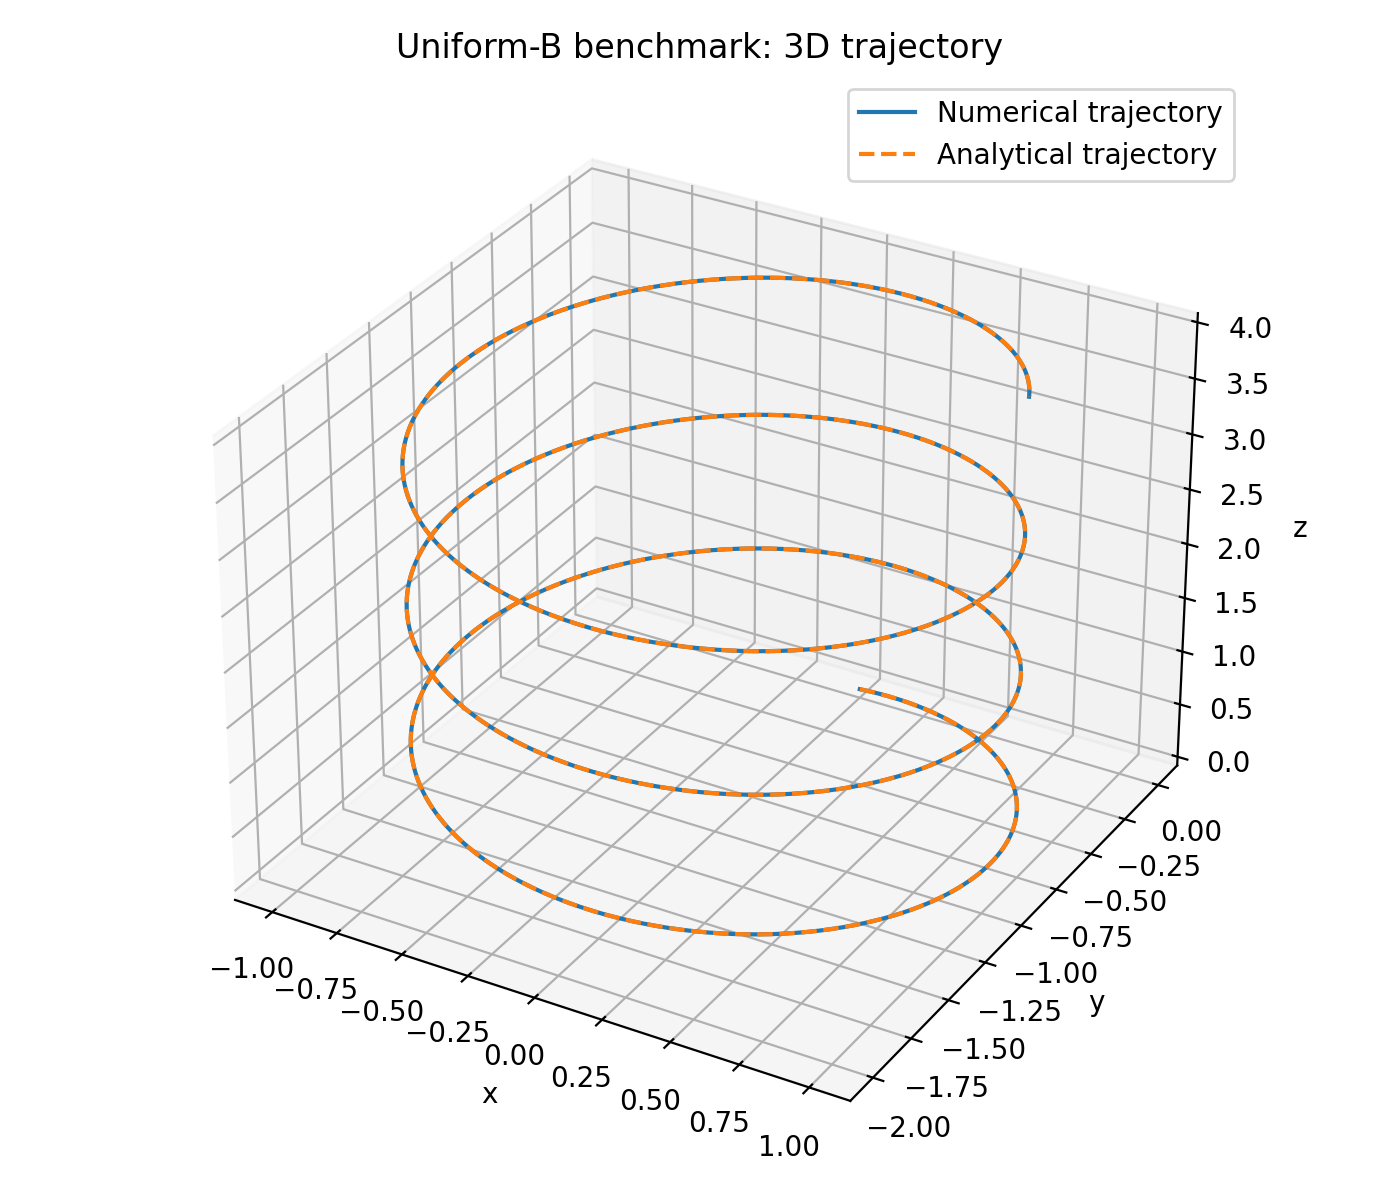
\includegraphics[width=\linewidth]{uniform_B_3d_trajectory.png}
        \caption{三维螺旋轨道。}
    \end{subfigure}\hfill
    \begin{subfigure}[t]{0.44\textwidth}
        \centering
        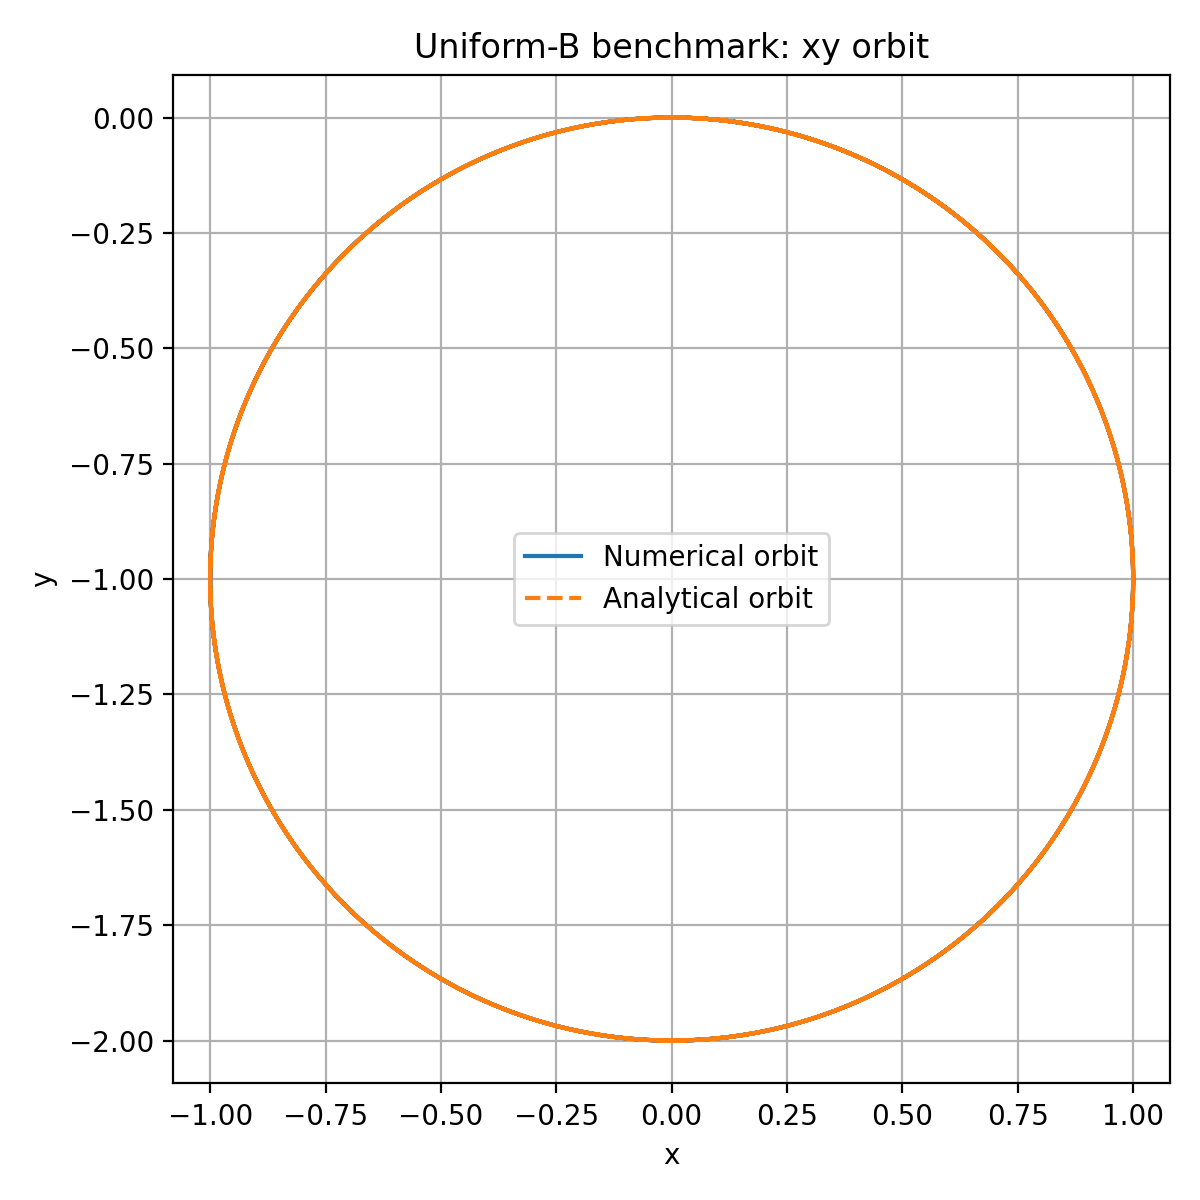
\includegraphics[width=\linewidth]{uniform_B_xy_orbit.png}
        \caption{垂直平面内的圆周轨道。}
    \end{subfigure}
    \caption{匀强磁场基准算例。在图示尺度下，数值轨道与解析轨道几乎完全重合。}
    \label{fig:uniformB}
\end{figure}

该算例验证了向量叉积、洛伦兹加速度、RK4 各级计算以及 CSV 输出，之后再引入更复杂的电磁场结构。

% --------------------------------------------------
\section{要求的漂移算例}
% --------------------------------------------------

\subsection{$E\times B$ 漂移}

对于均匀正交电磁场
\begin{equation}
    \vect{E}=E_0\hat{\vect{x}},\qquad
    \vect{B}=B_0\hat{\vect{z}},
\end{equation}
导引中心漂移速度为
\begin{equation}
    \boxed{\vE=\frac{\vect{E}\times\vect{B}}{B^2}}
    =-\frac{E_0}{B_0}\hat{\vect{y}}.
    \label{eq:exb}
\end{equation}
该漂移与粒子的质量和电荷大小无关。当 $E_0=0.1$、$B_0=1$ 时，理论漂移速度为 $v_{E,y}=-0.1$。对数值导引中心做线性拟合得到 $-0.10000000$，相对差约为 $1.1\times10^{-13}$。完整的数值粒子轨道与精确全轨道解在位置上也达到约 $10^{-9}$ 的一致性。

\begin{figure}[H]
    \centering
    \begin{subfigure}[t]{0.39\textwidth}
        \centering
        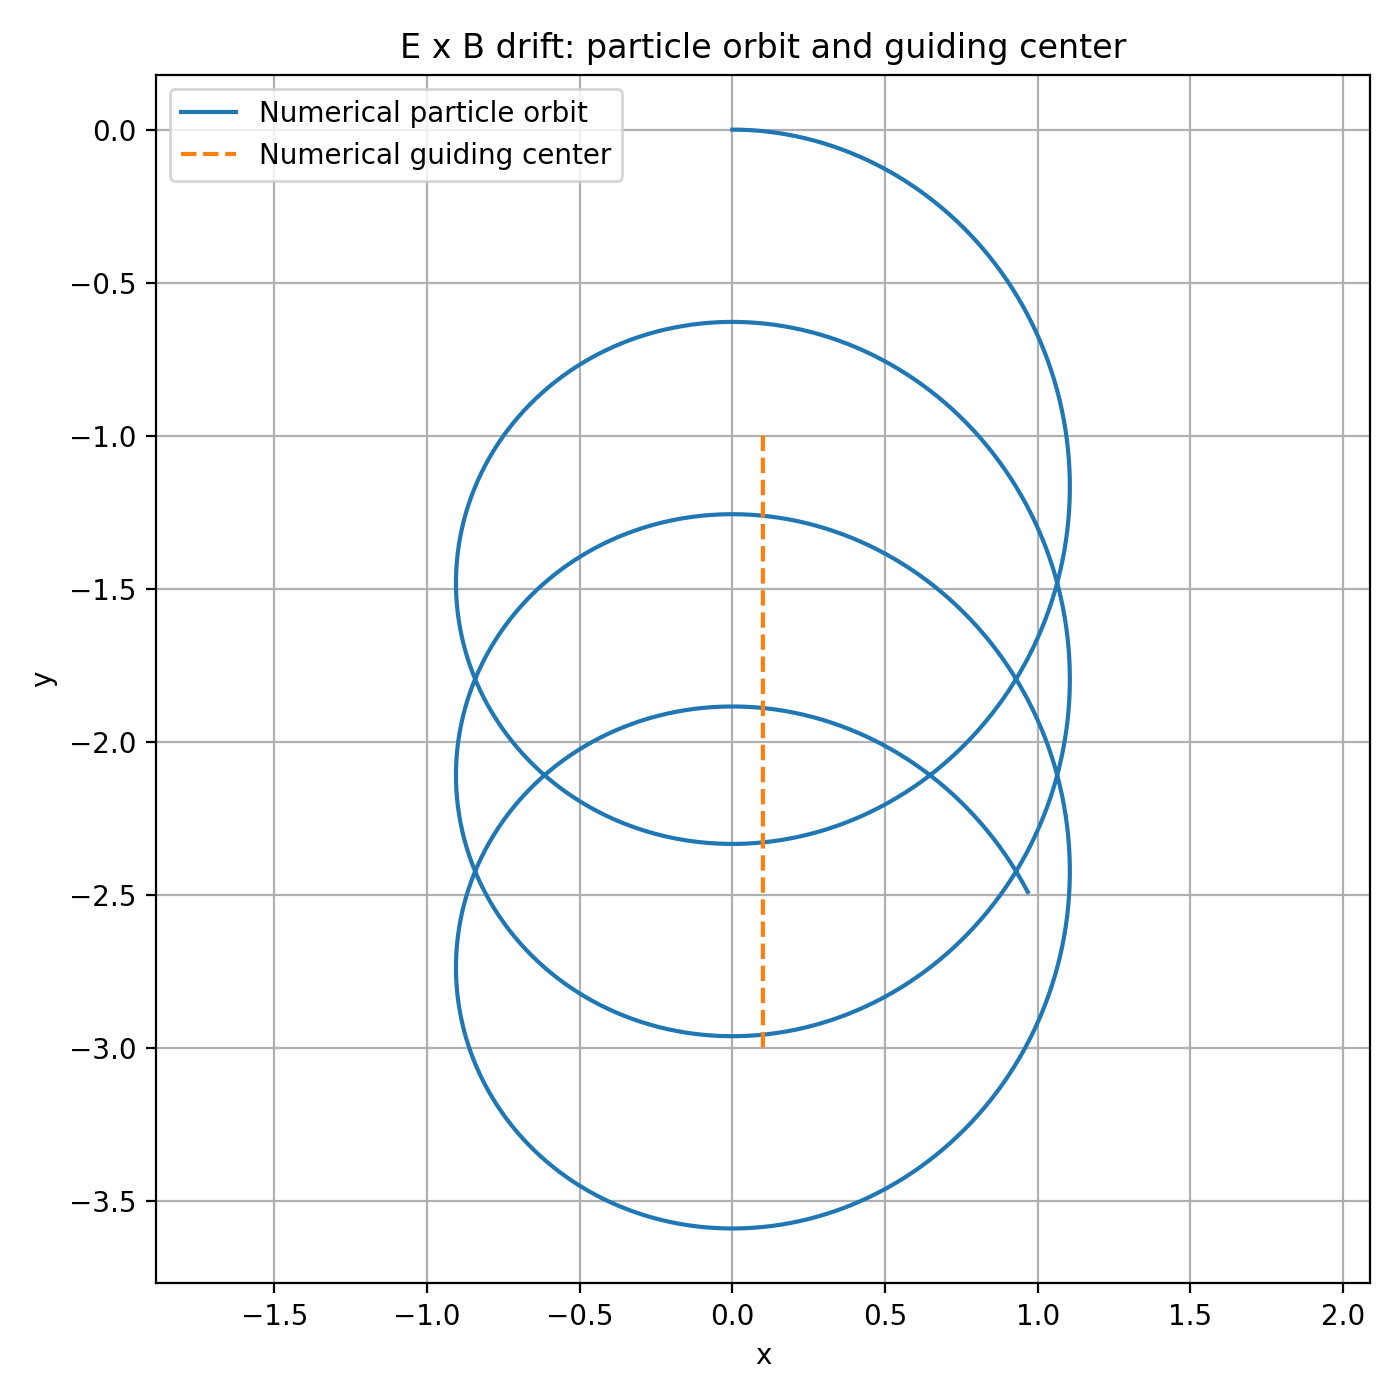
\includegraphics[width=\linewidth]{exb_xy_orbit.png}
        \caption{横向漂移上叠加的回旋运动。}
    \end{subfigure}\hfill
    \begin{subfigure}[t]{0.59\textwidth}
        \centering
        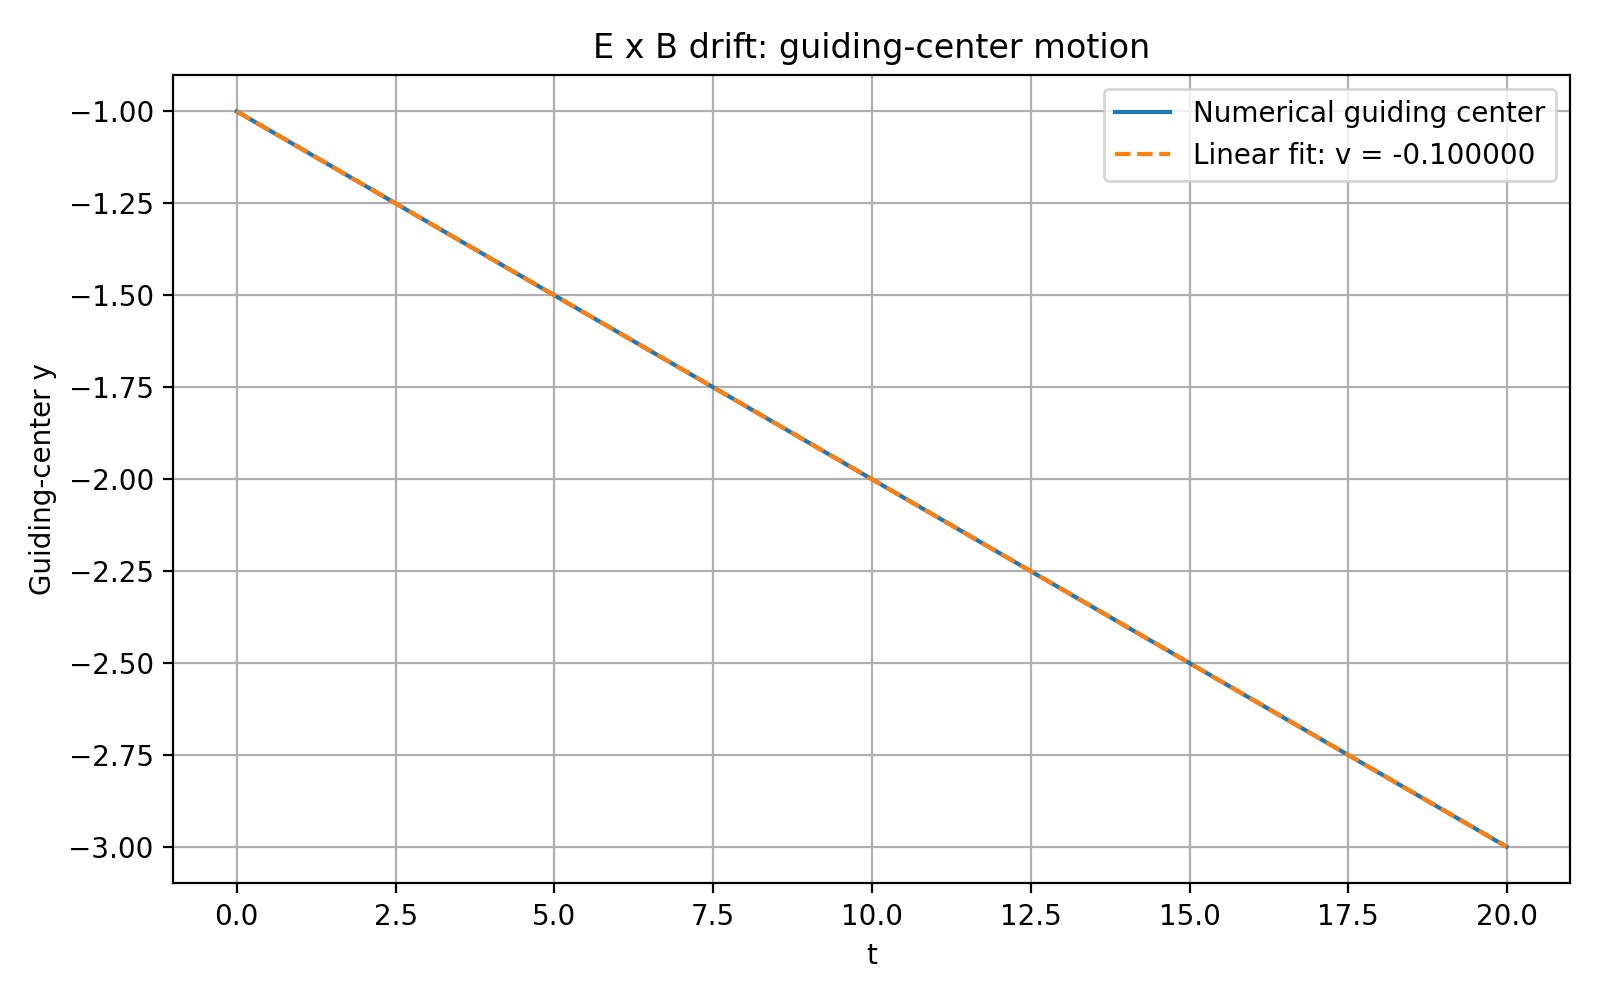
\includegraphics[width=\linewidth]{exb_guiding_center.png}
        \caption{导引中心位移及线性拟合。}
    \end{subfigure}
    \caption{$\vect{E}\times\vect{B}$ 漂移。C++ 运动方程中没有显式加入漂移公式，但完整轨道自然产生了理论导引中心速度。}
    \label{fig:exb}
\end{figure}

\subsection{磁场梯度漂移}

为了单独研究磁场强度梯度，选取
\begin{equation}
    \vect{B}(x)=B_0(1+gx)\hat{\vect{z}},\qquad \vect{E}=0,
    \label{eq:gradbfield}
\end{equation}
其中 $g=0.05$。由于 $B_z$ 仅依赖 $x$ 而不依赖 $z$，同时 $B_x=B_y=0$，因此该磁场满足 $\nabla\cdot\vect{B}=0$。

磁矩和一阶磁场梯度漂移分别为
\begin{equation}
    \mu=\frac{m v_\perp^2}{2B},
    \qquad
    \boxed{\vgradB=\frac{\mu}{qB^2}\vect{B}\times\nabla B}.
    \label{eq:gradb}
\end{equation}
初始时 $\rhL=1$，磁场变化的特征尺度为
\begin{equation}
    L_B=\frac{B}{|\nabla B|}=20,
    \qquad
    \epsilon_B=\frac{\rhL}{L_B}=0.05.
\end{equation}
因此在一次回旋轨道尺度内，磁场只发生较小变化，一阶导引中心理论应当具有较好的精度。理论给出 $v_{\nabla B,y}=0.025000$，数值结果为 $0.02506606$，相对差为 $0.264\%$。

\begin{figure}[H]
    \centering
    \begin{subfigure}[t]{0.42\textwidth}
        \centering
        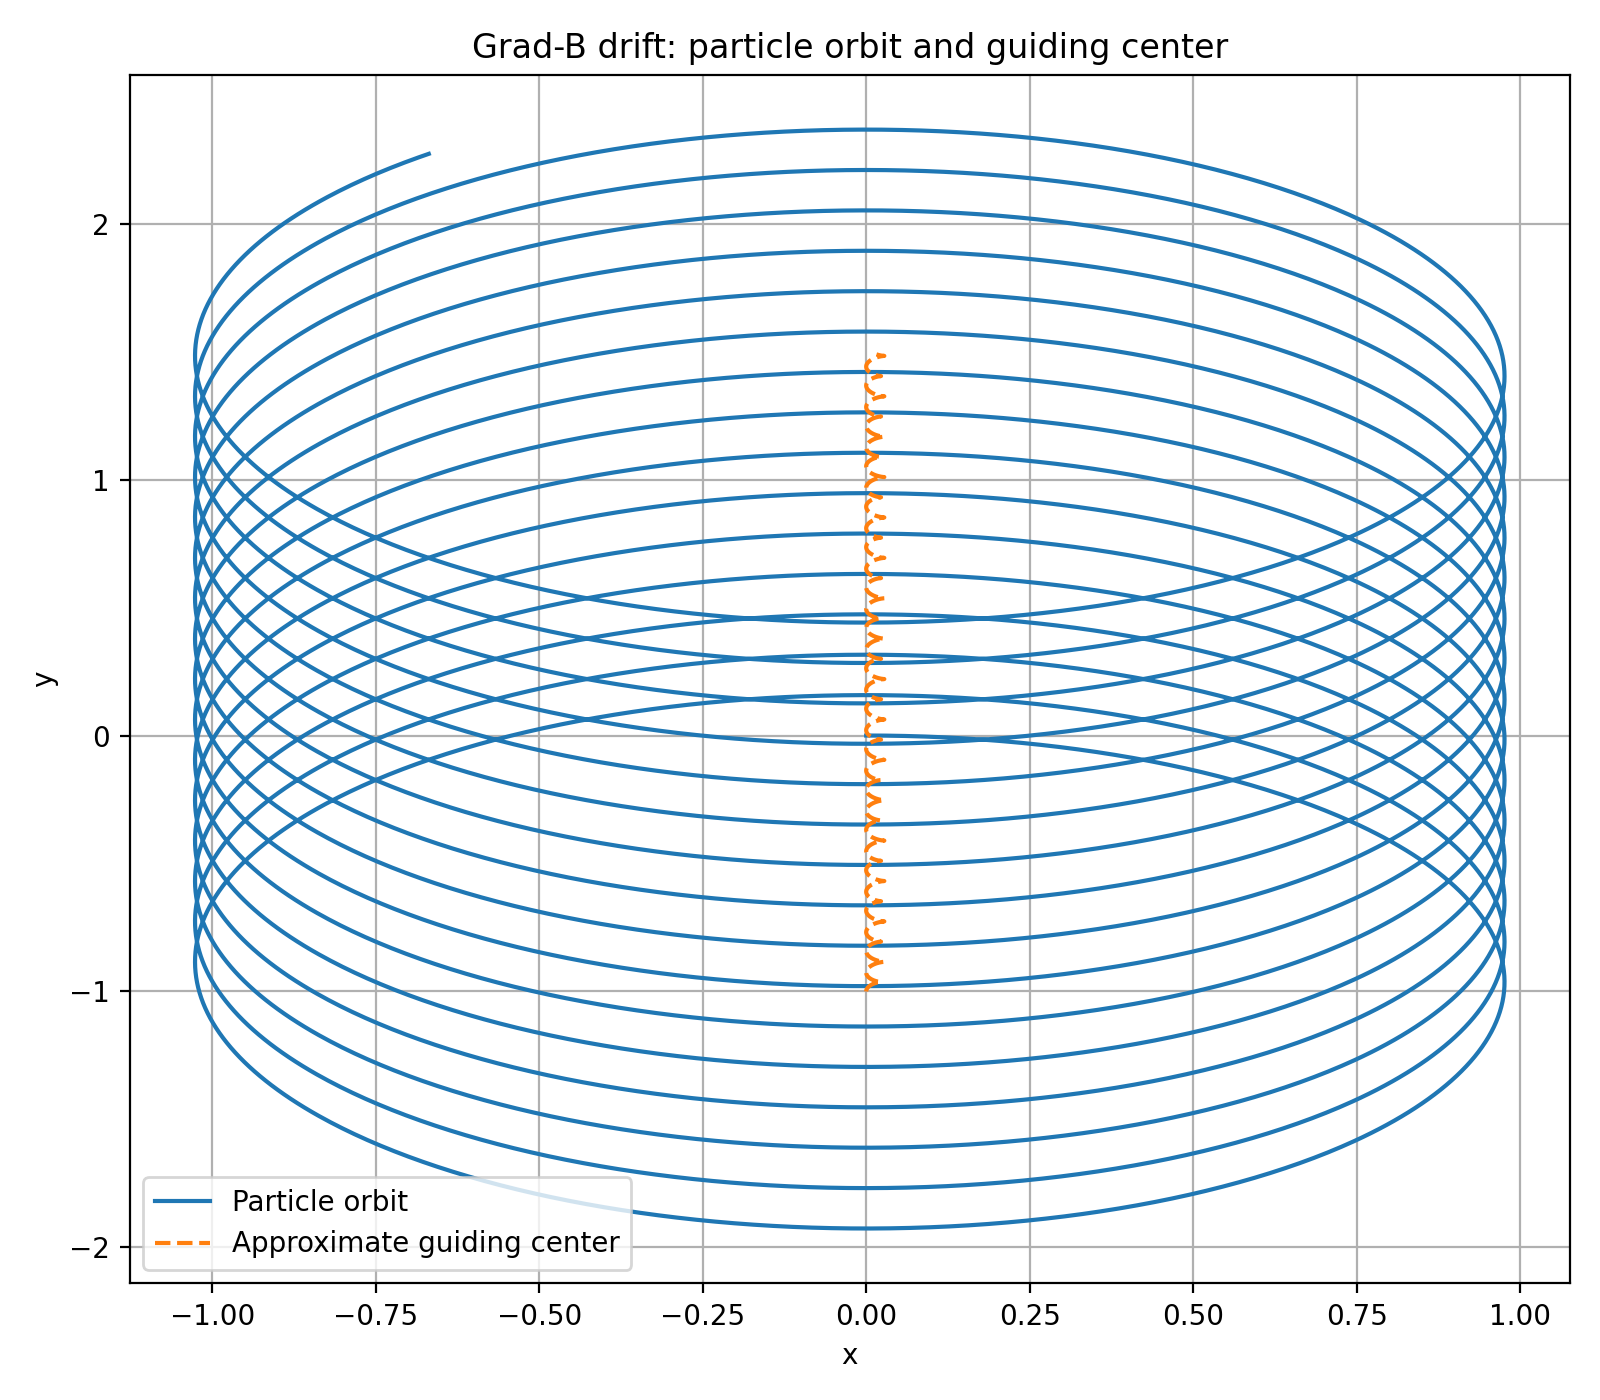
\includegraphics[width=\linewidth]{gradB_xy_orbit.png}
        \caption{粒子轨道与近似导引中心。}
    \end{subfigure}\hfill
    \begin{subfigure}[t]{0.56\textwidth}
        \centering
        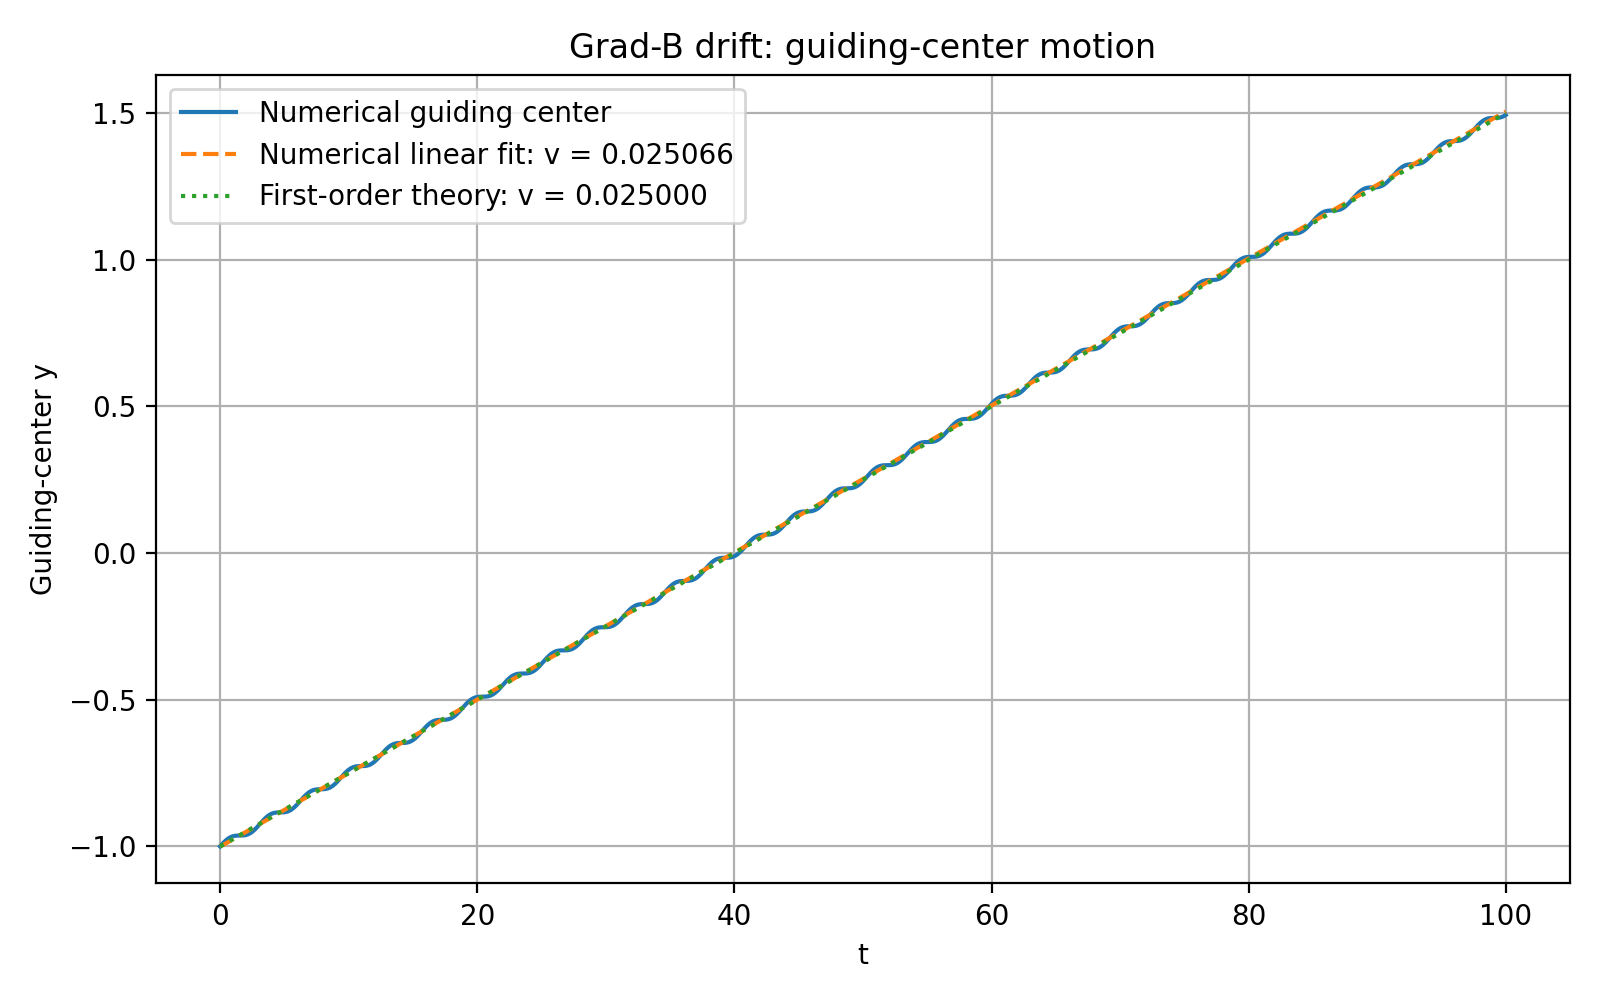
\includegraphics[width=\linewidth]{gradB_guiding_center.png}
        \caption{数值漂移与一阶理论的比较。}
    \end{subfigure}
    \caption{弱非均匀磁场中的磁场梯度漂移。}
    \label{fig:gradb}
\end{figure}

由于 $\vect{E}=0$，粒子的动能应保持不变。数值计算中动能的最大相对误差为 $1.35\times10^{-10}$。瞬时诊断量 $\mu=m v_\perp^2/(2B)$ 在回旋时间尺度上存在约 $5.4\%$ 的最大调制；绝热不变量的物理含义对应的是缓慢变化或回旋平均后的磁矩，而不是有限半径轨道上每一个瞬时位置处的数值都严格恒定。

\begin{figure}[H]
    \centering
    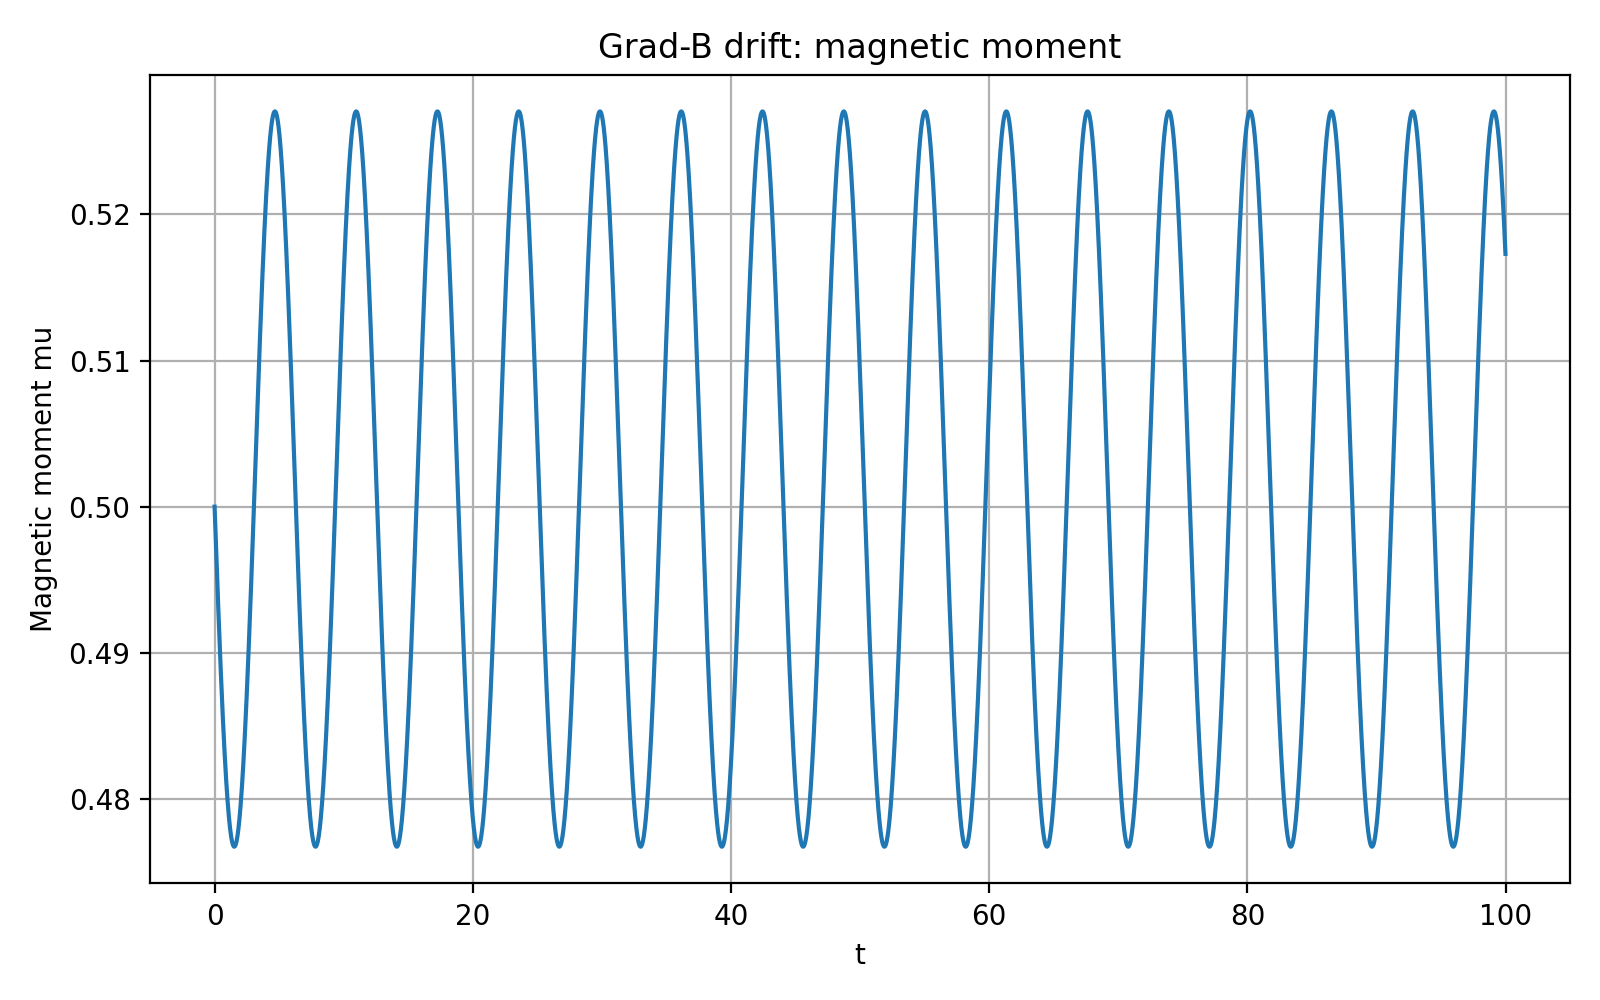
\includegraphics[width=0.68\textwidth]{gradB_magnetic_moment.png}
    \caption{磁场梯度算例中的瞬时磁矩。振荡发生在快速回旋尺度，而长期漂移保持为慢过程。}
    \label{fig:gradb_mu}
\end{figure}

\subsection{曲率漂移}

为了研究曲率而不同时引入 $\nabla|B|$，采用磁场强度恒定的方位向磁场：
\begin{equation}
    \vect{B}=B_0\hat{\vect{e}}_\phi
    =B_0\left(-\frac{y}{R},\frac{x}{R},0\right),
    \qquad R=\sqrt{x^2+y^2}.
    \label{eq:curvaturefield}
\end{equation}
该磁场的磁力线为圆，且 $|\vect{B}|=B_0$；除圆柱轴线外，满足 $\nabla\cdot\vect{B}=0$。对于圆形磁力线，其曲率向量为
\begin{equation}
    \vect{\kappa}=(\vect{b}\cdot\nabla)\vect{b}
    =-\frac{\hat{\vect{e}}_R}{R},
\end{equation}
一阶曲率漂移为
\begin{equation}
    \boxed{
    \vc=\frac{m v_\parallel^2}{qB}\,\vect{b}\times\vect{\kappa}
    }.
    \label{eq:curvdrift}
\end{equation}
在 $R_c=10$、$v_\parallel=1$、$v_\perp=0.2$ 的条件下，理论预测 $v_{c,z}=0.100000$。数值测得的导引中心速度为 $0.09727577$，对应 $2.72\%$ 的差异。导引中心半径的相对变化约保持在 $5\times10^{-12}$ 以内，动能守恒误差约为 $6\times10^{-12}$。

\begin{figure}[H]
    \centering
    \begin{subfigure}[t]{0.44\textwidth}
        \centering
        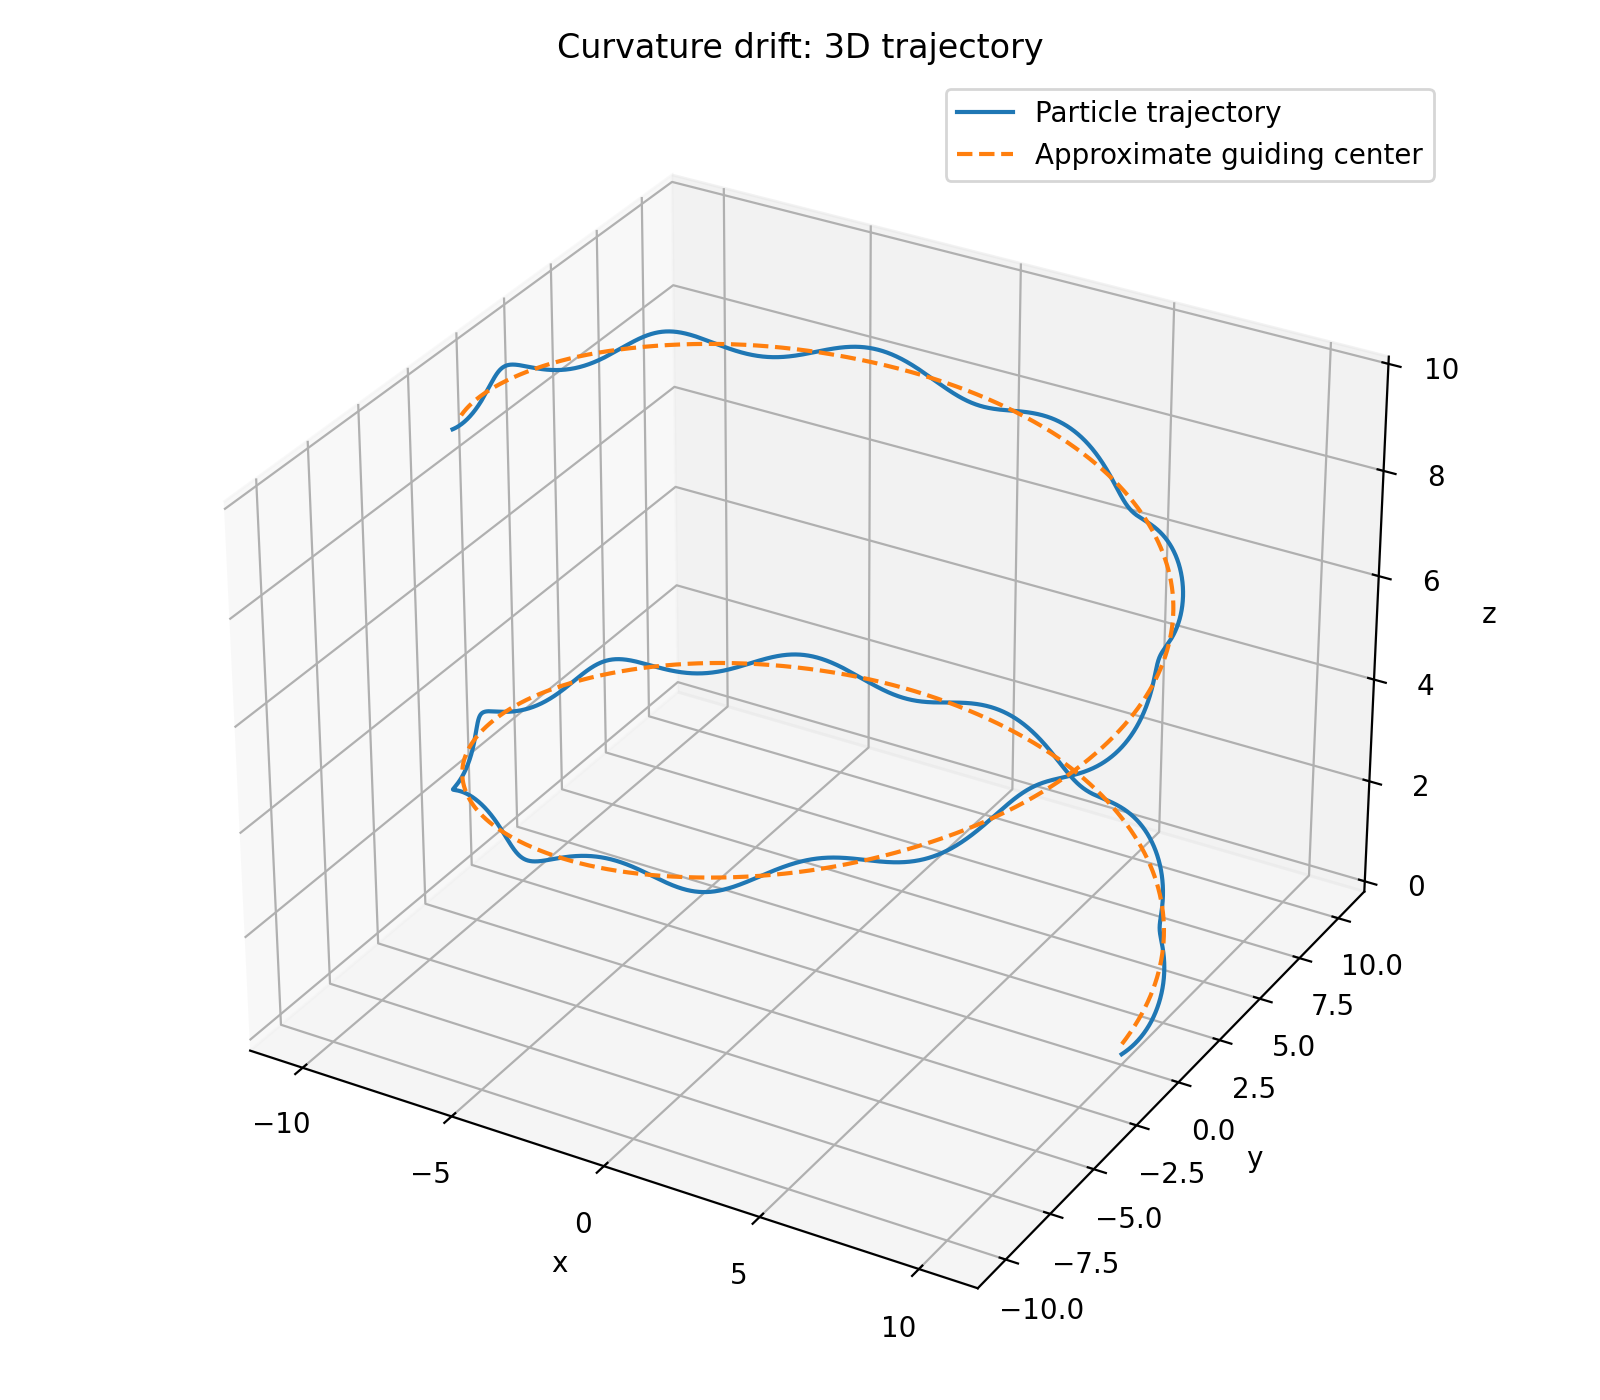
\includegraphics[width=\linewidth]{curvature_3d_trajectory.png}
        \caption{粒子轨道与导引中心轨道。}
    \end{subfigure}\hfill
    \begin{subfigure}[t]{0.54\textwidth}
        \centering
        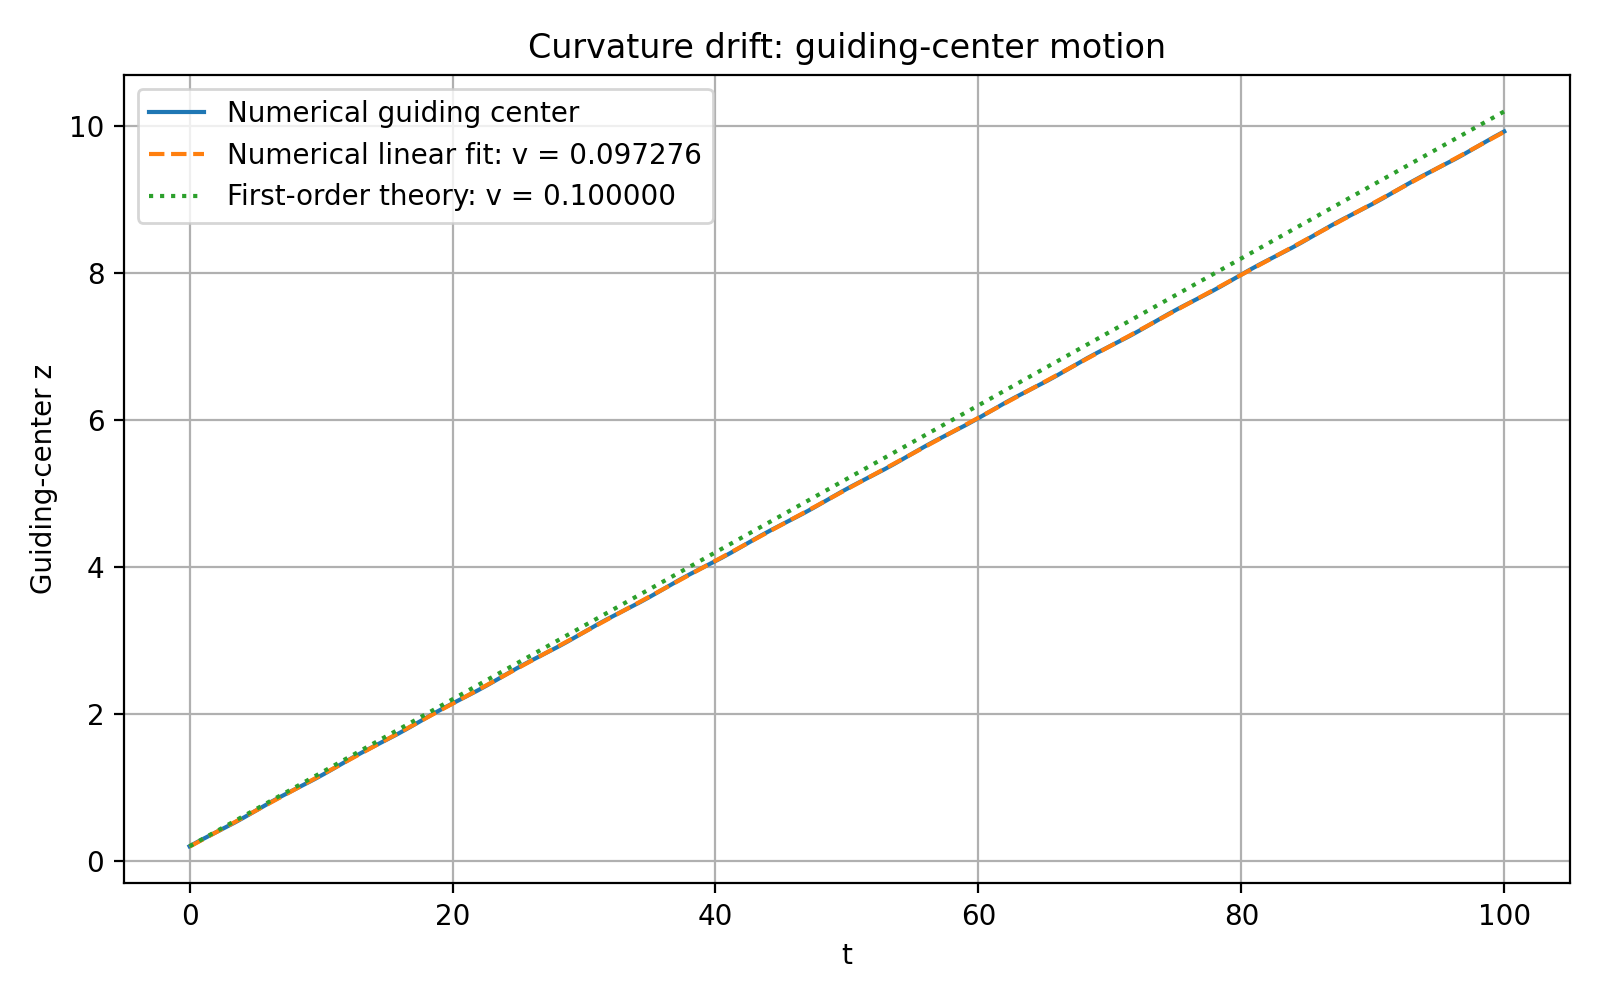
\includegraphics[width=\linewidth]{curvature_guiding_center.png}
        \caption{$z$ 方向漂移：数值结果与理论比较。}
    \end{subfigure}
    \caption{由圆形、恒定磁场强度的磁力线产生的曲率漂移。}
    \label{fig:curvature}
\end{figure}

\subsection{空间非均匀电场与有限拉莫尔半径修正}

非均匀电场算例采用
\begin{equation}
    \vect{E}(x)=E_0\cos(kx)\hat{\vect{x}},
    \qquad
    \vect{B}=B_0\hat{\vect{z}},
    \label{eq:nonuniformefield}
\end{equation}
其中 $E_0=0.02$、$k=0.4$。该电场为静电场，其势函数为
\begin{equation}
    \phi(x)=-\frac{E_0}{k}\sin(kx).
\end{equation}
粒子的拉莫尔半径为 $\rhL=1$，因此 $k\rhL=0.4$。由于拉莫尔半径不是零，粒子在一次回旋过程中会经过不同的 $x$ 位置，从而采样不同的 $E_x$。因此，零拉莫尔半径极限下仅在导引中心位置计算局域 $E\times B$ 漂移的近似需要加入有限拉莫尔半径（finite-Larmor-radius, FLR）修正。当 $k\rhL\ll1$ 时，
\begin{equation}
    \left\langle\vE\right\rangle
    \simeq
    \left(1-\frac{k^2\rhL^2}{4}\right)
    \frac{\vect{E}(\vect{R}_{gc})\times\vect{B}}{B^2}.
    \label{eq:flrsecondorder}
\end{equation}
对于未受扰的圆形回旋轨道，完整的回旋平均与贝塞尔因子 $J_0(k\rhL)$ 成正比。分析脚本通过对回旋角直接数值平均来计算同一结果，因此不需要额外的特殊函数库。

若忽略 FLR 效应，局域 $E\times B$ 预测为 $-0.020000$；二阶 FLR 近似给出 $-0.019200$；直接回旋平均给出 $-0.01920796$。完整轨道模拟得到
\begin{equation}
    v_{gc,y}^{\rm num}=-0.01920650.
\end{equation}
因此，数值模拟与零拉莫尔半径的局域 $E\times B$ 近似相差 $3.97\%$，但与直接回旋平均仅相差 $0.00764\%$。这一结果清楚地表明，该差异来自真实的 FLR 物理效应，而不是数值积分误差。

\begin{figure}[H]
    \centering
    \begin{subfigure}[t]{0.44\textwidth}
        \centering
        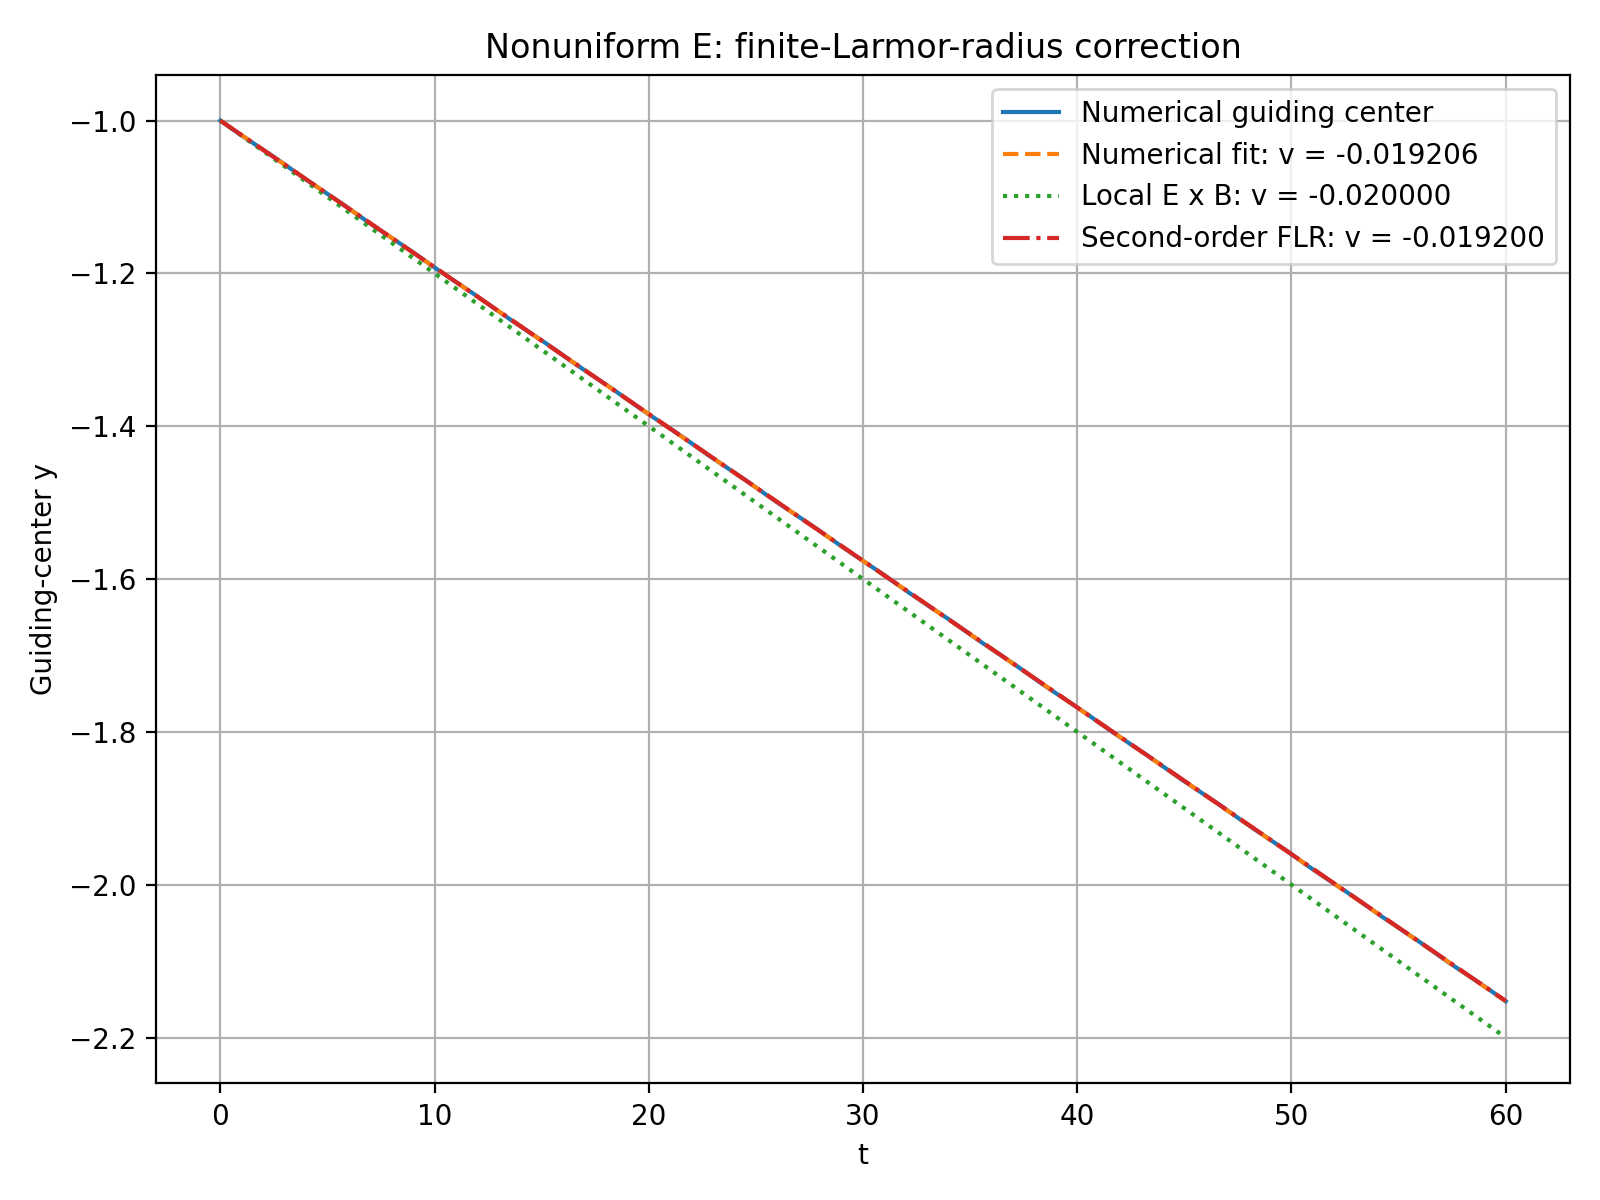
\includegraphics[width=\linewidth]{nonuniform_E_guiding_center.png}
        \caption{完整轨道漂移与局域及 FLR 预测的比较。}
    \end{subfigure}\hfill
    \begin{subfigure}[t]{0.54\textwidth}
        \centering
        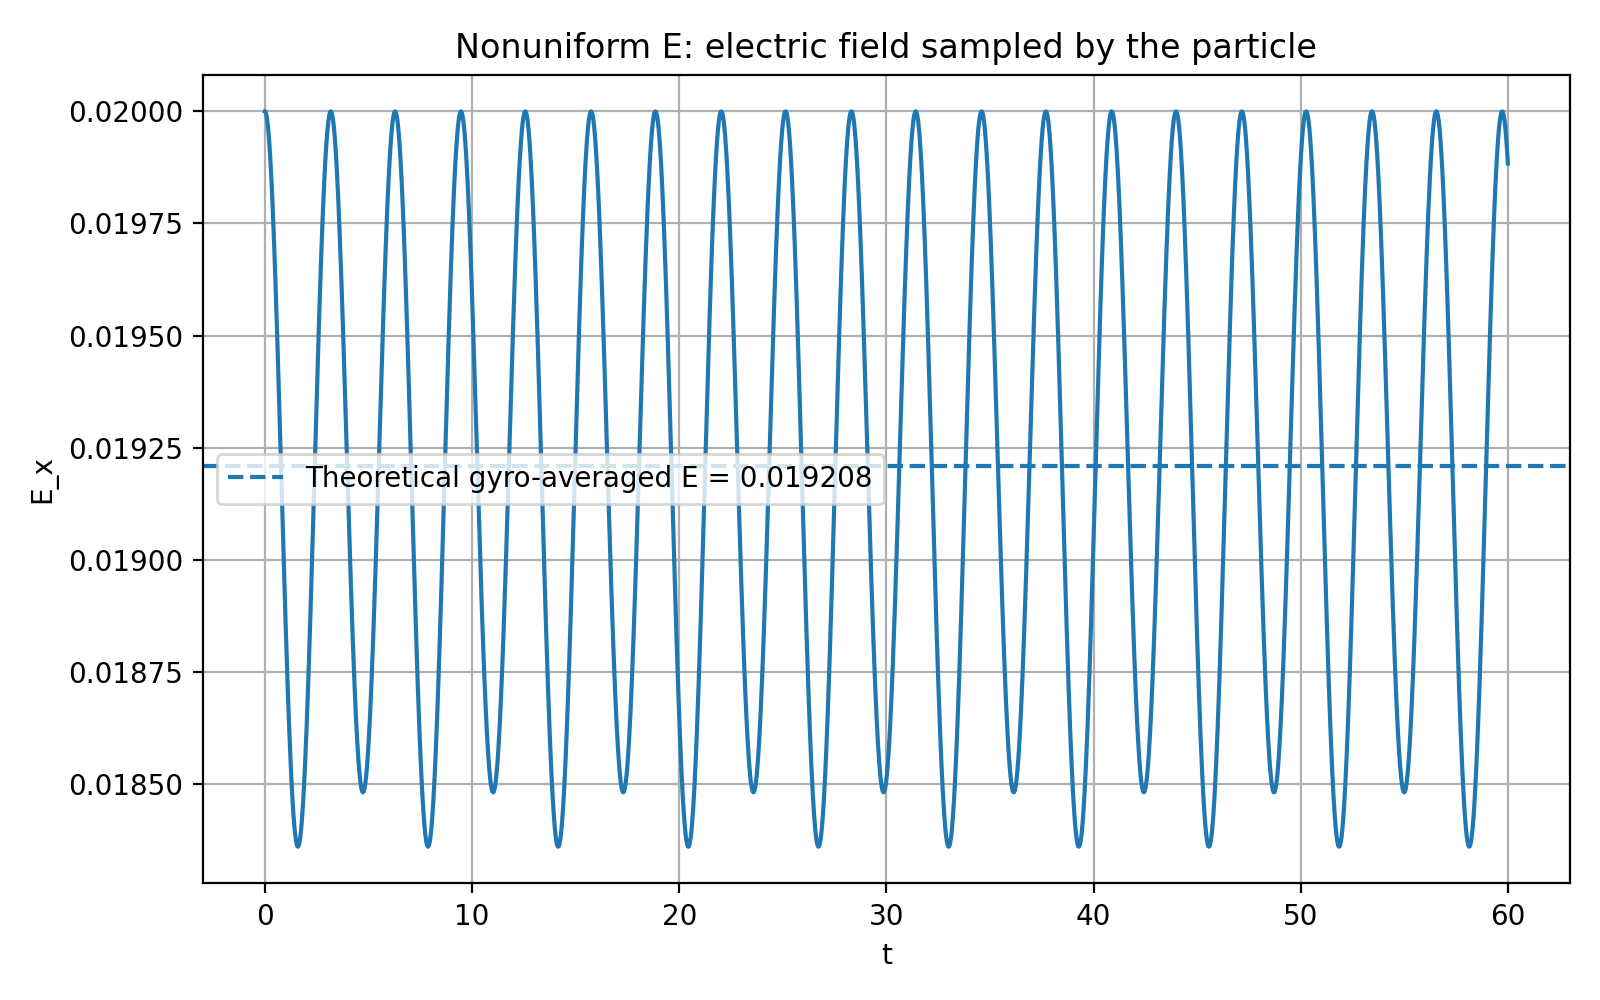
\includegraphics[width=\linewidth]{nonuniform_E_sampled_field.png}
        \caption{粒子在回旋轨道上采样到的电场。}
    \end{subfigure}
    \caption{空间变化静电场中的有限拉莫尔半径效应。}
    \label{fig:nonuniformE}
\end{figure}

导引中心的 $X$ 坐标在数值精度范围内保持不变。此外，静电情况下的总能量
\begin{equation}
    \mathcal{H}=K+q\phi
\end{equation}
最大相对误差为 $8.11\times10^{-11}$。

\subsection{极化漂移}

最后一个算例采用缓慢变化的垂直电场
\begin{equation}
    \vect{E}(t)=E_0\cos(\omega_E t)\hat{\vect{x}},
    \qquad
    \vect{B}=B_0\hat{\vect{z}},
    \label{eq:polarizationfield}
\end{equation}
其中 $E_0=0.2$、$\omega_E=0.05$。由于 $\Ohm=1$，
\begin{equation}
    \frac{\omega_E}{\Ohm}=0.05\ll1,
\end{equation}
说明外加电场的变化频率远低于粒子的回旋频率，符合推导极化漂移时所采用的缓变条件。一阶近似下，
\begin{align}
    v_{E,y}(t) &= -\frac{E_0}{B_0}\cos(\omega_E t),\\
    \boxed{
    v_{p,x}(t)=\frac{m}{qB_0^2}\frac{dE_x}{dt}
    =-\frac{mE_0\omega_E}{qB_0^2}\sin(\omega_E t)
    }.
    \label{eq:polarization}
\end{align}
相应的一阶速度振幅分别为 $|v_E|=0.2000$ 和 $|v_p|=0.0100$。

由于外加频率是有限值而不是严格趋近于零，精确的慢响应与一阶漂移理论之间存在因子
\begin{equation}
    \frac{1}{1-(\omega_E/\Ohm)^2}=1.00250627,
\end{equation}
因此 $y$ 方向慢响应振幅为 $0.20050125$，$x$ 方向为 $0.01002506$。对于该算例，受迫全轨道方程还可以精确求解，因此能够对 C++ 轨道进行非常严格的独立验证。数值解与精确解之间的位置最大误差约为 $3.2\times10^{-11}$，速度最大误差约为 $1.1\times10^{-11}$。

\begin{figure}[H]
    \centering
    \begin{subfigure}[t]{0.49\textwidth}
        \centering
        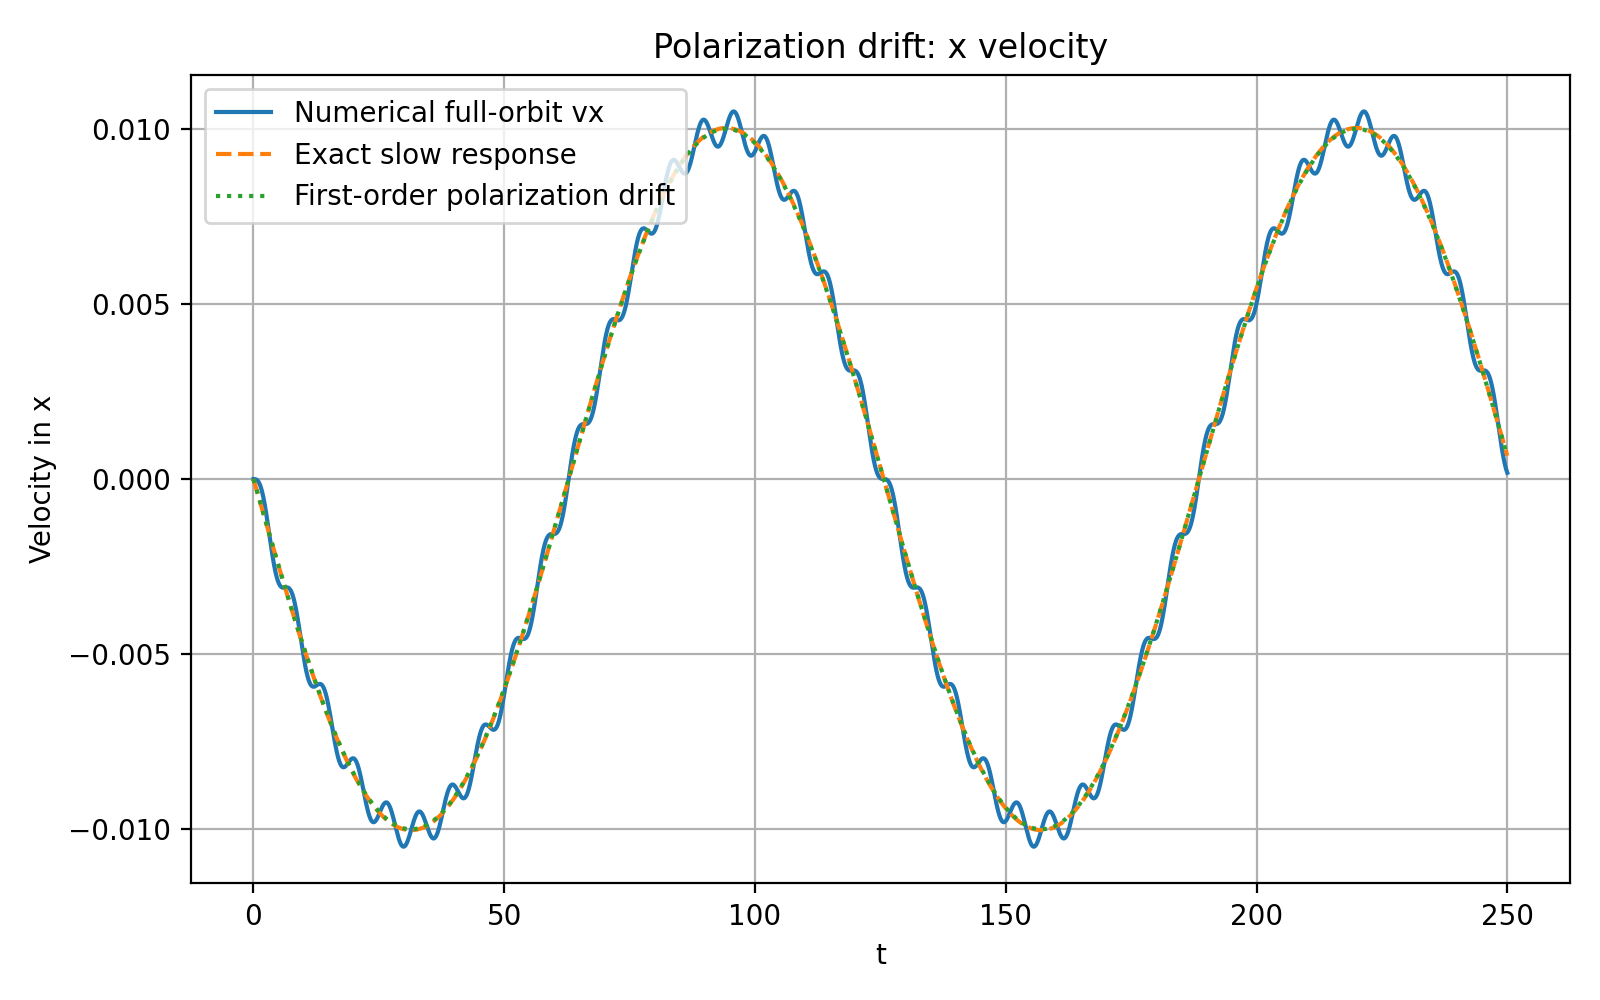
\includegraphics[width=\linewidth]{polarization_velocity_x.png}
        \caption{$x$ 方向的极化响应。}
    \end{subfigure}\hfill
    \begin{subfigure}[t]{0.49\textwidth}
        \centering
        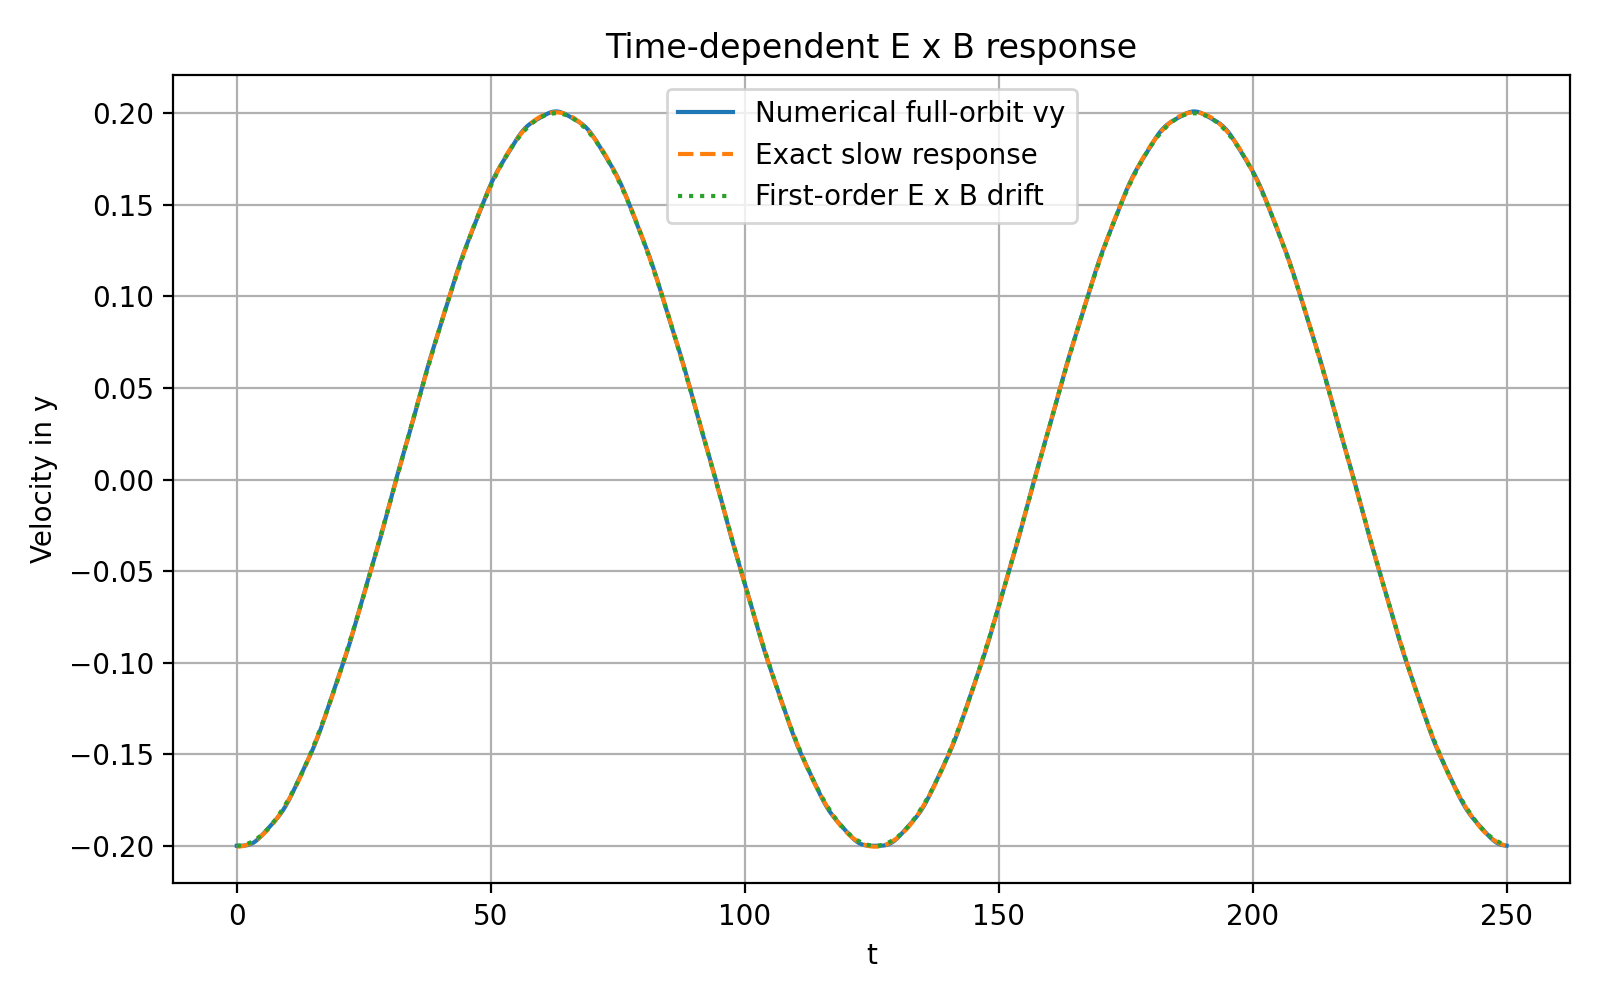
\includegraphics[width=\linewidth]{polarization_exb_velocity_y.png}
        \caption{$y$ 方向随时间变化的 $E\times B$ 响应。}
    \end{subfigure}
    \caption{极化漂移基准算例。完整轨道遵循精确的有限频率响应，而一阶漂移理论给出了预期的低频极限。}
    \label{fig:polarization_velocity}
\end{figure}

\begin{figure}[H]
    \centering
    \begin{subfigure}[t]{0.41\textwidth}
        \centering
        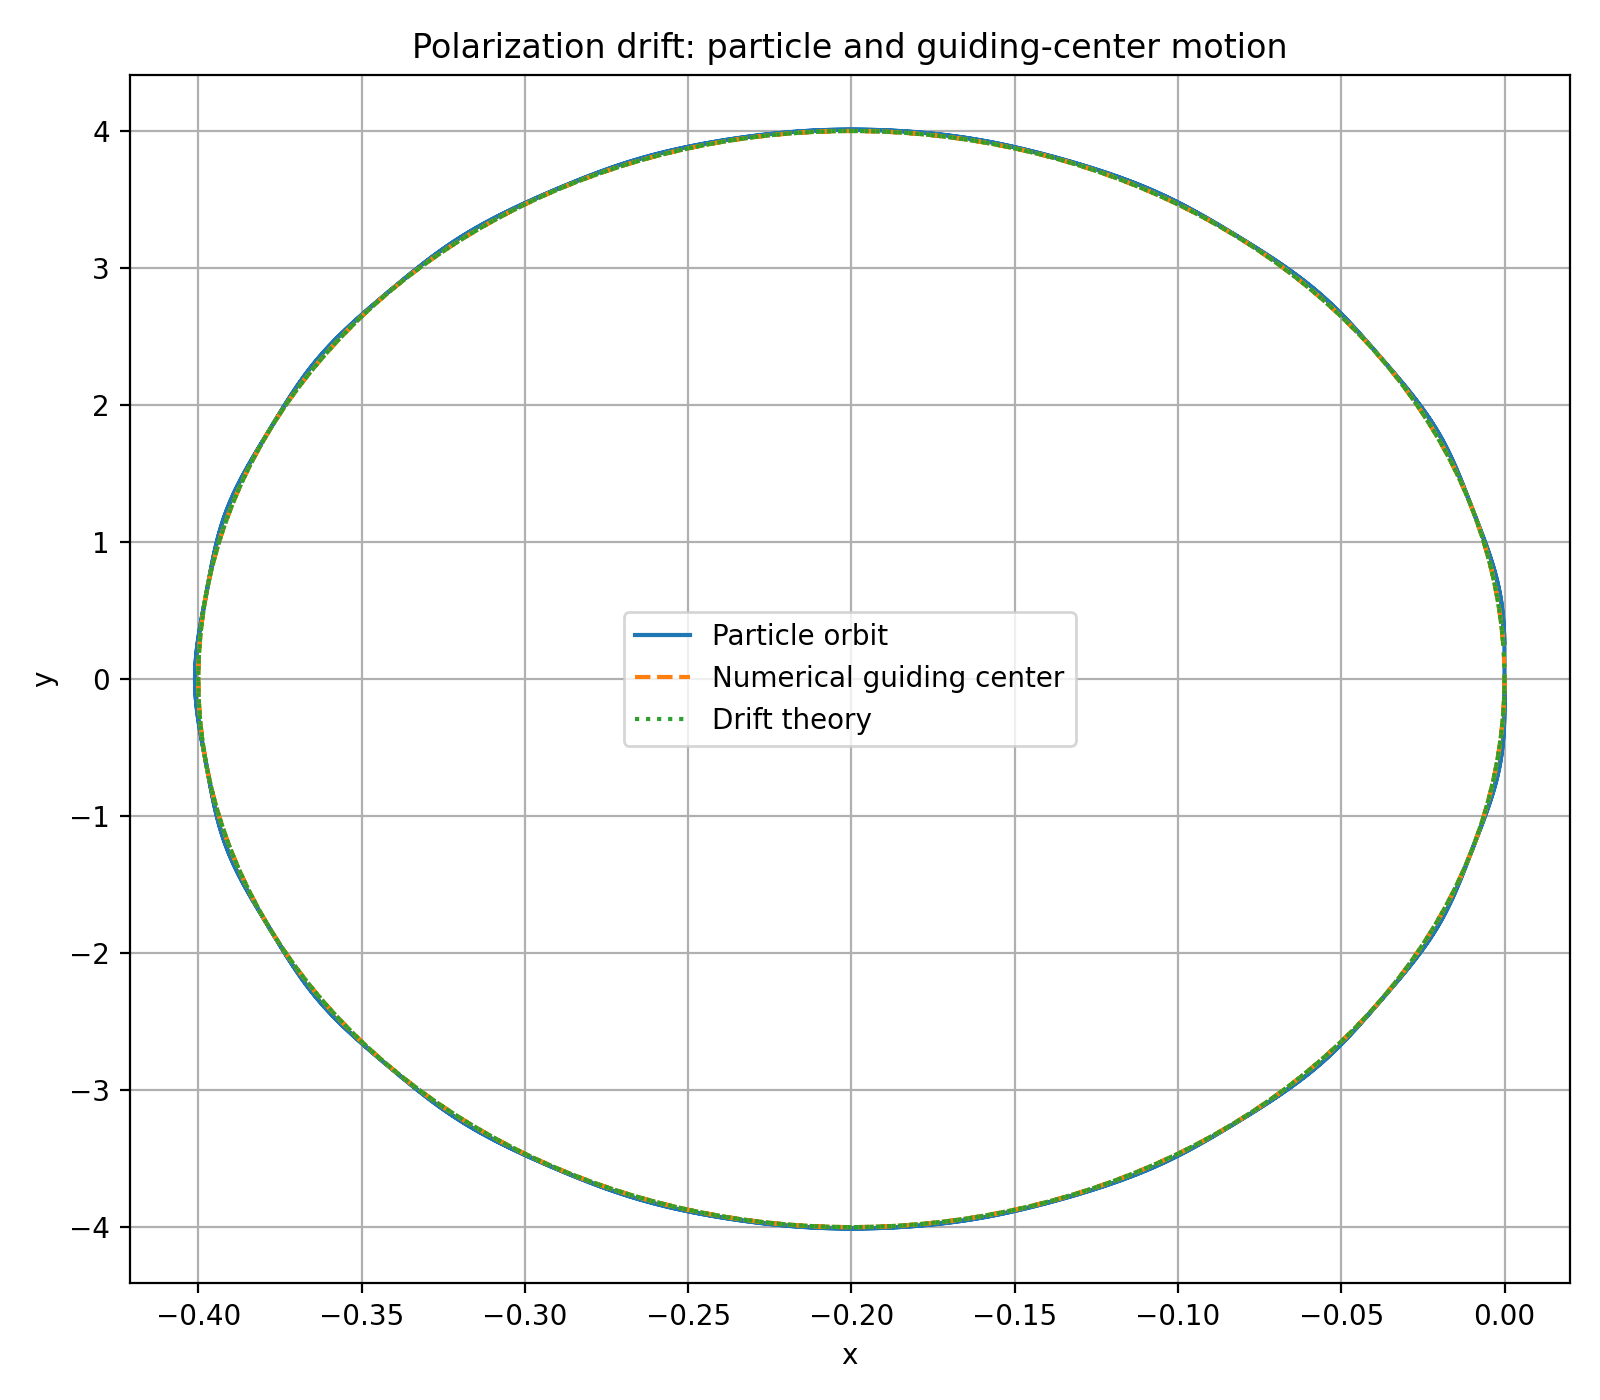
\includegraphics[width=\linewidth]{polarization_xy_motion.png}
        \caption{垂直平面轨道：数值解与精确解。}
    \end{subfigure}\hfill
    \begin{subfigure}[t]{0.57\textwidth}
        \centering
        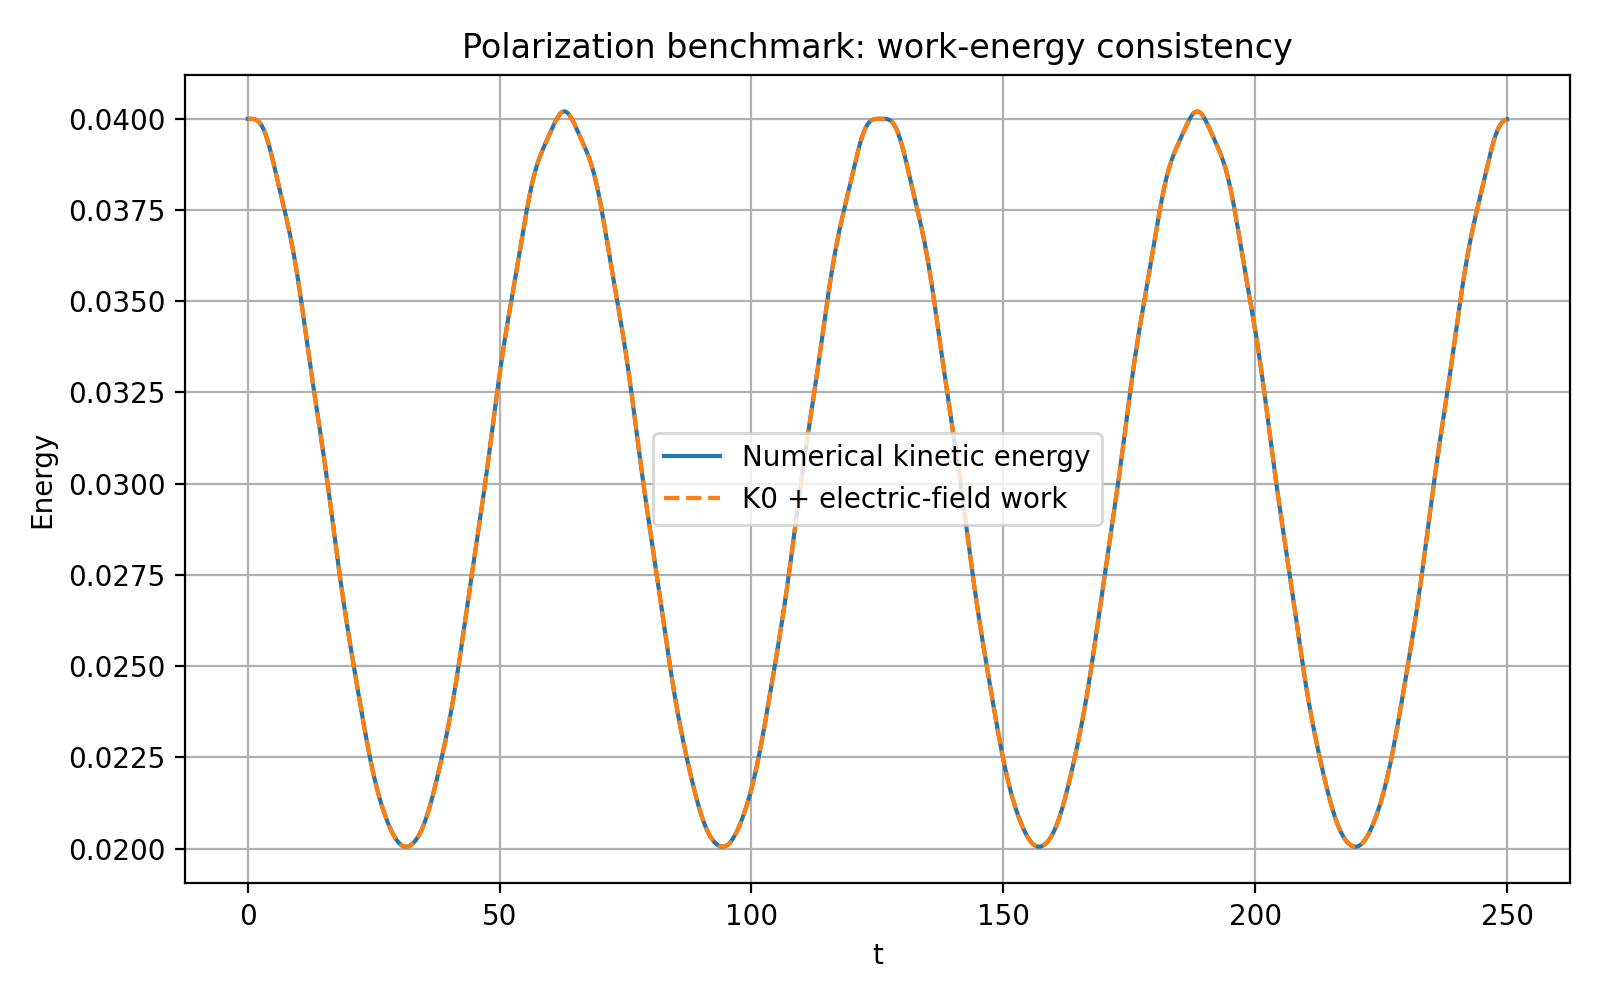
\includegraphics[width=\linewidth]{polarization_energy.png}
        \caption{动能与电场做功。}
    \end{subfigure}
    \caption{极化漂移算例的独立检验。功--能关系 $K(t)-K(0)=\int q\vect{E}\cdot\vect{v}\,dt$ 的绝对能量误差约为 $1.7\times10^{-9}$。}
    \label{fig:polarization_checks}
\end{figure}

% --------------------------------------------------
\section{定量结果汇总}
% --------------------------------------------------

\begin{table}[H]
    \centering
    \small
    \caption{数值结果与相应理论预测的比较。}
    \resizebox{\textwidth}{!}{%
    \begin{tabular}{lllll}
        \toprule
        \textbf{算例} & \textbf{参考量} & \textbf{理论值} & \textbf{数值值} & \textbf{差异} \\
        \midrule
        $E\times B$ & $v_{E,y}$ & $-0.10000000$ & $-0.10000000$ & $1.1\times10^{-13}$（相对） \\
        磁场梯度 & $v_{\nabla B,y}$ & $0.02500000$ & $0.02506606$ & $0.264\%$ \\
        曲率 & $v_{c,z}$ & $0.10000000$ & $0.09727577$ & $2.72\%$ \\
        非均匀 $E$ & 回旋平均 $v_y$ & $-0.01920796$ & $-0.01920650$ & $0.00764\%$ \\
        极化 & 精确全轨道 & 解析轨道 & 数值轨道 & $\sim10^{-11}$ 轨道误差 \\
        \bottomrule
    \end{tabular}}
    \label{tab:summary}
\end{table}

具有精确解的基准算例（匀强 $B$、均匀正交电磁场以及受迫极化算例）主要用于检验数值积分器本身。磁场梯度和曲率算例则用于比较完整粒子轨道与降阶的一阶导引中心理论，因此其百分数量级的差异不应被解释为 RK4 的数值误差。非均匀电场算例尤其清楚地体现了这种区别：数值结果与零拉莫尔半径近似有明显差异，但与包含有限拉莫尔半径效应的回旋平均结果高度一致。

% --------------------------------------------------
\section{讨论}
% --------------------------------------------------

这些模拟展示了导引中心理论所依赖的尺度分离：快速的回旋运动叠加在更缓慢的横跨磁场运动之上。不过，各算例中慢漂移的物理来源并不相同。

\begin{itemize}
    \item $\vect{E}\times\vect{B}$ 漂移是两种电荷符号都共有的精确漂移，其速度不依赖 $m$ 或 $q$。
    \item 磁场梯度漂移和曲率漂移依赖粒子性质，分别源于磁场强度的不均匀性和磁力线几何曲率。它们的一阶公式属于渐近导引中心理论，而不是完整轨道的精确解。
    \item 空间非均匀电场体现了有限拉莫尔半径物理：粒子会在整个回旋轨道上采样电场，因此当 $k\rhL$ 不是零时，仅在导引中心位置计算 $\vect{E}$ 并不足够。
    \item 极化漂移是一种由时间变化引起的惯性修正。在低频极限下，其速度比随时间变化的 $E\times B$ 运动小一个约为 $\omega_E/\Ohm$ 的因子。
\end{itemize}

本文选择的场模型尽可能单独隔离每一种物理效应。磁场梯度算例所用磁场满足 $\nabla\cdot\vect{B}=0$；曲率算例保持 $|B|$ 恒定，因此不会把曲率漂移与磁场梯度漂移混合。非均匀电场为静电场，因此还可以独立检验 $K+q\phi$ 的守恒性。

% --------------------------------------------------
\section{结论}
% --------------------------------------------------

本文使用 C++17 实现了一个紧凑的三维带电粒子全轨道模拟程序，通过洛伦兹方程和四阶 Runge--Kutta 方法完成数值积分。所有要求的算例均使用同一个积分器，仅改变预设电磁场和初始条件。独立的 Python 脚本用于解析验证、导引中心重构、守恒量诊断、拟合和可视化。

五种要求的漂移现象均被成功再现：
\begin{itemize}
    \item 均匀正交电磁场产生了预期的 $\vect{E}\times\vect{B}$ 漂移；
    \item 弱磁场梯度产生了预期的磁场梯度漂移；
    \item 圆形且磁场强度恒定的磁力线产生了曲率漂移；
    \item 空间变化的静电场显示了预期的有限拉莫尔半径修正；
    \item 缓慢随时间变化的电场产生了极化漂移以及随时间变化的 $\vect{E}\times\vect{B}$ 响应。
\end{itemize}

对于存在精确解析解的算例，数值全轨道与解析解达到约 $10^{-9}$--$10^{-11}$ 的一致性，说明数值积分误差远小于非均匀场情况下导引中心近似本身带来的物理误差。因此，本项目直接数值展示了常见漂移速度如何从完整的洛伦兹动力学中自然产生，而不是作为额外的运动方程被人为加入模拟。

% --------------------------------------------------
\begin{thebibliography}{9}

\bibitem{Chen2016}
F. F. Chen,
\textit{Introduction to Plasma Physics and Controlled Fusion},
3rd ed., Springer, 2016.

\end{thebibliography}

\end{document}
